\chapter{Экспериментальное исследование оптических частотных гребенок в кристаллических микрорезонаторах} \label{chapt3}

\section{Изготовление кристаллических микрорезонаторов методом алмазного точения}

В литературе были продемонстрированы следующие способы изготовления микрорезонаторов:

\begin{itemize}
  \item Плавление в пламени водородной горелки для микросфер из плавленого кварца.
  \item Выжигание мощным лазером $CO_2$ вращающейся заготовки.
  \item Механическое точение резонаторов.
  \item Различные литографические методы для изготовление интегральных микрорезонаторов.
\end{itemize}

В данной работе для изготовления всех микрорезонаторов из кристаллических материалов изучался и использовался метод алмазного точения с последующей полировкой алмазными суспензиями.

Общий внешний вид микрорезонаторов представлен на рис. \ref{cavity_scheme_big}. Основные характеристики микрорезонатора - это диаметр, толщина цилиндра и радиус закругления боковой поверхности цилиндра, где сосредоточено поле мод шепчущей галереи.  Размеры варьируются в следующих пределах: диаметр 100 мкм – 8 мм (в зависимости от необходимой ОСД $FSR= \frac{c}{2\pi Rn}$), толщина 0.1 мм – 2мм (в зависимости от толщины изначальной заготовки) и радиус закругления от 30 мкм до $R/2$ (где $R$ – радиус резонатора).

\begin{figure}[ht]
    \centering
  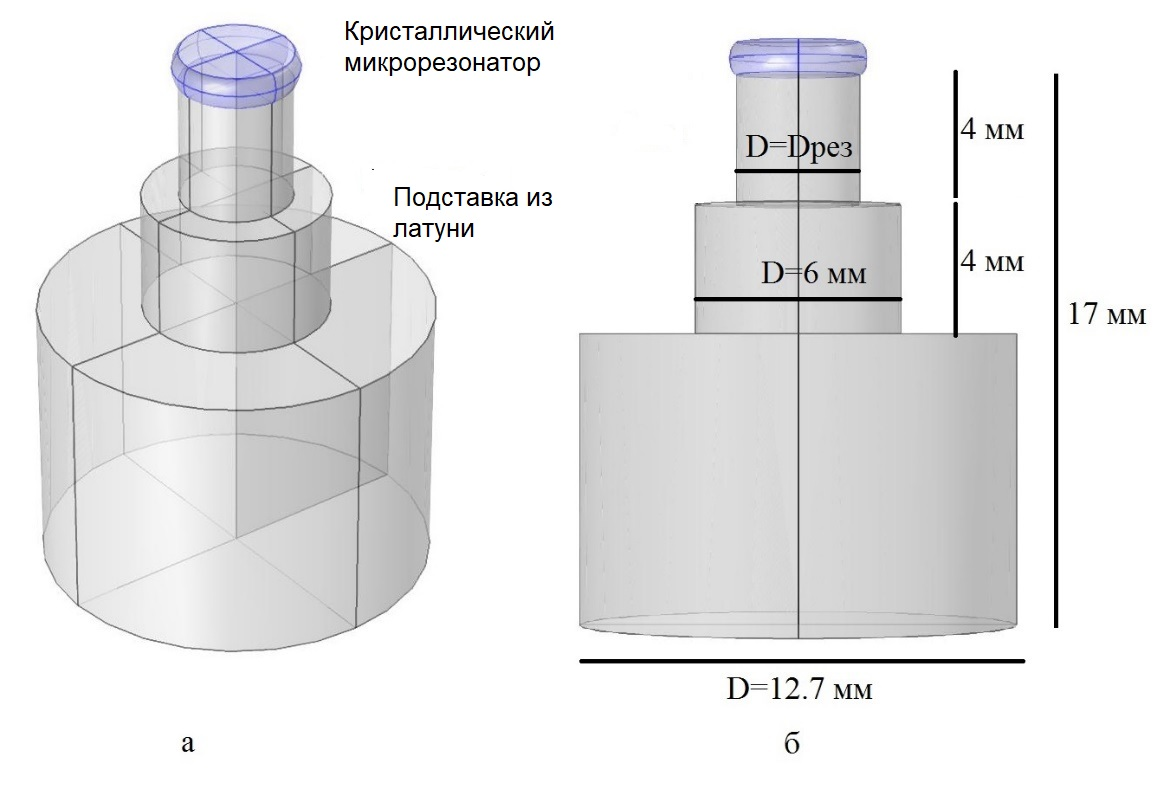
\includegraphics[width=0.5\linewidth]{cavity_scheme_big}
  \caption{Внешний вид кристаллического микрорезонатора и пьедестала: а – 3D вид, б – сечение XZ}
  \label{cavity_scheme_big}
\end{figure}

Для изготовления микрорезонатора с модами шепчущей галереи (ММШГ) использовались кристаллические пластины фторида магния ($MgF_2$), фторида кальция ($CaF_2$), фторида бария ($BaF_2$), фторида стронция ($SrF_2$), фторида лития ($LiF$), ниобата лития ($LiNbO_3$), танталата лития ($LiTaO_3$), кремния ($Si$), кристаллического кварца ($SiO_2$) и ряда других матералов (TGG).

Кристаллические микрорезонаторы из вышеуказанных материалов не могут быть изготовлены путем нагрева и обжига пламенем или мощным $CO_2$ лазером. Также пока не разработаны литографические способы их изготовления с необходимым качеством поверхности. Поэтому используется механическая обработка заготовок кристаллов в два этапа: точение алмазным резцом на прецизионном станке и последующая полировка алмазными пленками и суспензиями.

Ниже приведена последовательность действий, необходимых для изготовления микрорезонатора:

\begin{itemize}
  \item Наклеивание цилиндрической заготовки кристалла на латунную подставку с помощью УФ клея.
  \item Вытачивание цилиндра заданного диаметра алмазным резцом на станке алмазного точения (может выполняться изношенным резцом).
  \item Вытачивание на цилиндре микрорезонатора с заданной геометрией с помощью острого алмазного резца и программы для ЧПУ.
  \item Очистка микрорезонатора с помощью салфетки, смоченной в изопропаноле или метаноле.
  \item Проверка качества получившейся поверхности в микроскоп для обнаружения возможных шероховатостей, а также с помощью профилометра и методом проверки добротности.
\end{itemize}

Хотя техника алмазного точения единственной точкой (SPDT, single point diamond turning) давно используется в большом количестве приложений, строгой теории для оптимального процесса точения нет. В процессе работы были экспериментально найдены оптимальные параметры для процесса точения.

Для алмазного точения использовался прецизионный станок с ЧПУ DAC ALM Lathe (рис. \ref{lathe}). Станок имеет прецизионный шпиндель на воздушных подшипниках и $2$ подвижные оси X,Y также на воздушных подшипниках. Точность подачи Х,Y специфицирована в $<10$ нм. Станок управляется с помощью программ, написанных на специально разработанном языке DSL. Станок оборудован высокоточным датчиком расстояния (LVDT), который измеряет расстояние по оси Y до момента касания заготовки. Также в комплекте к станку идет датчик высоты (профилометр), который измеряет изменение высоты с точностью до $0.1$ мкм. При двустороннем точении используется датчик, наносящий тонкие угловые отметки, позволяющие калибровать начало отсчета по оси C (угловое вращение шпинделя). Станок оборудован осциллирующим резцом, который синхронизируется с вращением шпинделя, и позволяет изготавливать асферические поверхности, а также выступы на фронтальной поверхности заготовки.

\begin{figure}[ht]
  \begin{minipage}[ht]{0.49\linewidth}\centering
    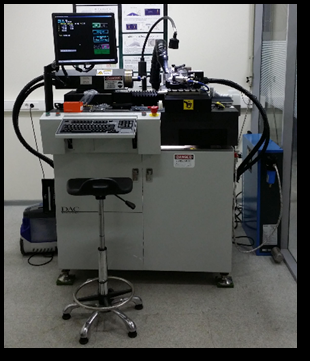
\includegraphics[width=1\linewidth]{lathe}
  \end{minipage}
  \hfill
  \begin{minipage}[ht]{0.49\linewidth}\centering
    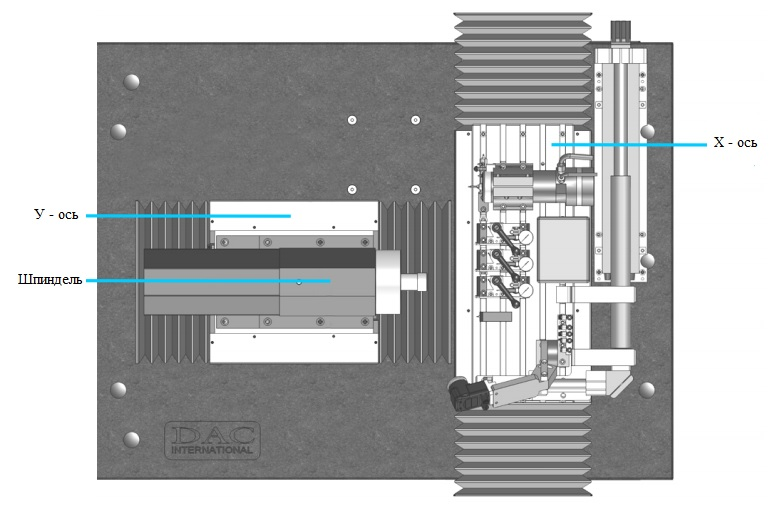
\includegraphics[width=1\linewidth]{lathe_top_view}
  \end{minipage}
  \caption{Прецизионный станок алмазного точения DAC ALM Lathe. Направление осей X,Y.}
  \label{lathe}
\end{figure}

Для точения использовались поликристаллические алмазные резцы производства KY Diamonds следующих типов (рис. \ref{diamond_tools}): 1) с радиусом кривизны 500 мкм, рабочей дугой окружности в 120 градусов, с 0 углом наклона рабочего края, конический задний угол резца 10 градусов; 2) с радиусом кривизны 100 мкм, рабочей дугой окружности в 60 градусов, с -25 углом наклона рабочего края, цилиндрический задний угол резца 8 градусов; 3) острый резец невыдержанным радиусом кривизны 4 мкм, 0 угол наклона рабочего края. Резцы располагались в держателе перпендикулярно (или под углом 80 градусов) к оси вращения шпинделя со вставленным резонатором.

\begin{figure}[ht]
  \begin{minipage}[ht]{0.24\linewidth}\centering
    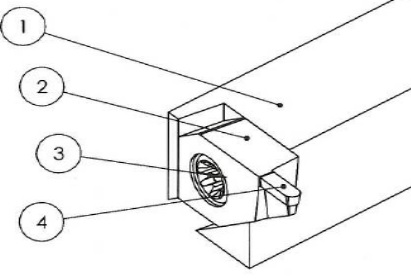
\includegraphics[width=1\linewidth]{tool1}
  \end{minipage}
  \hfill
  \begin{minipage}[ht]{0.24\linewidth}\centering
    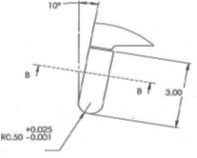
\includegraphics[width=1\linewidth]{tool2}
  \end{minipage}
  \hfill
  \begin{minipage}[ht]{0.24\linewidth}\centering
    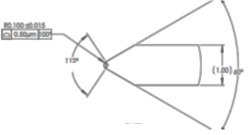
\includegraphics[width=1\linewidth]{tool3}
  \end{minipage}
  \hfill
  \begin{minipage}[ht]{0.24\linewidth}\centering
    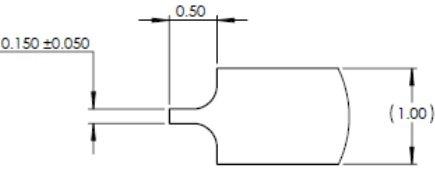
\includegraphics[width=1\linewidth]{tool4}
  \end{minipage}
  \caption{Чертежи используемых резцов.}
  \label{diamond_tools}
\end{figure}

Калибровка резцов проводилась по следующей методике:

\begin{itemize}
    \item В цангу вставляется заготовка (пластиковый цилиндр) диаметром 12.7 мм. Шпиндель подводится к калибруемому резцу. Выставляется на глаз отступ по оси Y до момента появления стружки (касания алмазного резца).
    \item Запускается программа, которая датчиком измеряет расстояние между фронтальной рабочей поверхностью до и после снятия слоя заданной толщины (например, 50 мкм). Точно зная это расстояние, окончательно калибруется зазор между датчиком расстояния LVDT и рабочей точкой резца.
    \item Запускается программа, наносящая штрих глубиной 1 мкм от края заготовки до ее центра (без вращения шпинделя). В оптический микроскоп (увеличение 40x) измеряется расстояние от центра заготовки до штриха (рис. \ref{tool_calibration}). Для правильной калибровки рабочая кромка резца изначально должна быть немного ниже центра. Используя датчик высоты, подстраивается высота калибруемого резца. Процедура повторяется до тех пор, пока штрих не будет проходить строго через центр заготовки.
    \item Проводится автоматическая калибровка расстояния по оси Х от рабочей точки алмазного резца до центра заготовки путем вытачивания трех концентрических окружностей: две при вращении шпинделя по часовой стрелке с одной стороны от центра, третья при вращении шпинделя в обратную сторону с другой стороны от центра. Далее измеряется получившееся расстояние между этими окружностями (с помощью датчика LVDT) и корректируется величина отступа между рабочей точкой резца и центром заготовки по оси X.
    \item В конце проводится калибровка расстояния по оси X до рабочей точки резца при точении цилиндра. Важно отметить, что точение фронтальной поверхности заготовки (перпендикулярно оси вращения шпинделя) и точение боковой поверхности цилиндра (параллельно оси вращения) осуществляется разными точками. Калибровка проводится путем вытачивания цилиндра заданного диаметра с последующим измерением получившегося диаметра с помощью микрометра. При необходимости расстояние по оси Х корректируется, и калибровка повторяется. Стоит подчеркнуть, что эта калибровка наименее точная из всех, т.к. погрешность микрометра при измерении диаметра цилиндра из мягкого пластика может составлять 5-10 мкм.
\end{itemize}


\begin{figure}[ht]
    \centering
  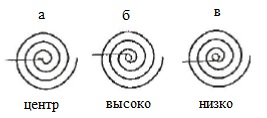
\includegraphics[width=0.5\linewidth]{tool_calibration}
  \caption{Результат калибровки высоты резца (правильная калибровка, резец высоко, резец низко).}
  \label{tool_calibration}
\end{figure}

Калибровка резцов осуществляется после каждой смены алмаза или при значительных дефектах обрабатываемых поверхностей.
Перед точением на станке из большой пластины материала резонатора вырезаются заготовки прямоугольной формы нужного малого размера. Для этого используется пила с алмазным диском, охлаждение производится специальной жидкостью.
Далее кристаллические заготовки наклеиваются на держатель (пьедестал) из латуни диаметром 12,7 мм, который соответствуют диаметру цанги на шпинделе станка. В работе использовались оптические клеи от производителя Norland Products (марки NOA 60, 61, 63, 65, 68), которые отвердевают при облучении УФ лампой. Клеи отличаются вязкостью в жидком виде, модулем упругости и твердостью в затвердевшем виде, оптическим показателем преломления и областью прозрачности. Все они не являются токопроводящими. Наилучший результат был достигнут с марками NOA 61, 65. Время облучения УФ лампой на длине 365 нм и мощностью 27 Вт/см$^2$ составляло 10 мин. Также использовались эпоксидная смола и этилцианакрилат, которые также давали хороший результат, но не позволяли долго центровать кристаллическую заготовку. Минимальный диаметр микрорезонатора, при котором не происходило отклеивание при точении, составил 700 мкм.
После точения микрорезонаторы могли быть переклеены на пьедестал меньшего диаметра. Все клеи размягчались и позволяли отклеить микрорезонатор при нагреве до 300-400 С. Также были испытаны двухкомпонентные клеи AremCo, который отвердевают за 24 часа при температуре 94 С, и выдерживают температуру нагревания до 400 С. Такой клей потенциально может использоваться при отжиге резонаторов.

Для центровки кристаллической заготовки в пьедестале вырезалось отверстие глубиной 0.5 мм и диаметром, позволяющим разместить в нем заготовку. В отверстие заливался клей, помещалась заготовка и облучалась УФ лампой. Проверка центровки и перпендикулярности плоскости кристалла и оси вращения шпинделя проводилась визуально с помощью микроскопической трубы, подвешенной над шпинделем станка.

Были написаны программы на языке DAC DSL для вытачивания из цилиндрических кристаллических заготовок микрорезонаторов ММШГ со следующими профилями боковой поверхности: угловая, сферическая, прямоугольный выступ. Параметры геометрии микрорезонатора настраиваются в широком диапазоне, ограниченном в основном геометрией самого алмазного резца.


\begin{figure}[ht]
  \begin{minipage}[ht]{0.49\linewidth}\centering
    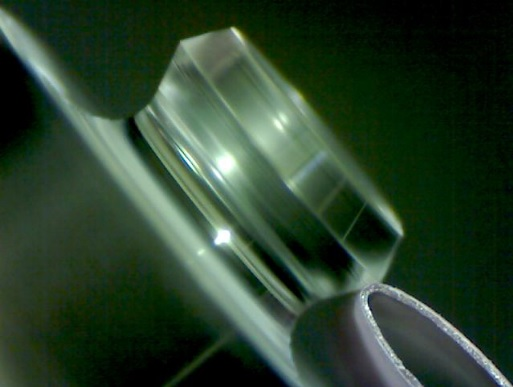
\includegraphics[width=1\linewidth]{cavity_fab_pad}
  \end{minipage}
  \hfill
  \begin{minipage}[ht]{0.49\linewidth}\centering
    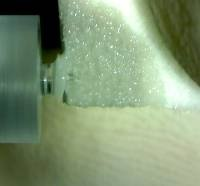
\includegraphics[width=1\linewidth]{cavity_fab_polishing}
  \end{minipage}
  \caption{Процесс ручной полировки алмазной шкуркой (слева) и алмазной суспензией (справа). Чистка резонатора проводилась на том же устройстве с использованием метилового спирта и салфеток Kimwipes.}
  \label{cavity_fab}
\end{figure}

\begin{figure}[ht]
\centering
  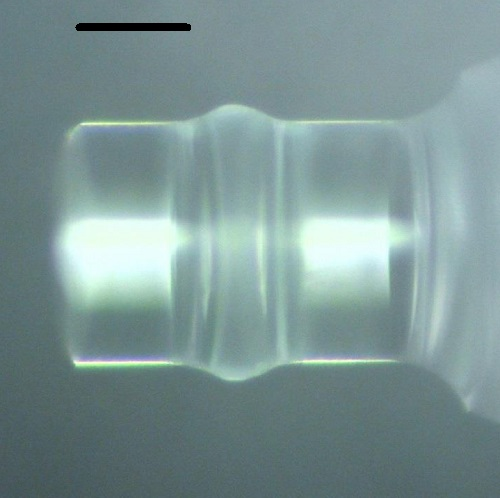
\includegraphics[width=0.5\linewidth]{cavity_fab_small}
  \caption{Микрорезонатор ММШГ ($MgF_2$) диаметром 250 мкм и радиусом кривизны боковой поверхности 50 мкм, выточенный с помощью программы DAC DSL.}
  \label{cavity_small}
\end{figure}

Алгоритм работы программы следующий:
\begin{itemize}
  \item Задаются начальные параметры (см рис. \ref{cavity_scheme})
  \begin{enumerate}
    \item диаметр заготовки (\texttt{blank\_diameter}),
    \item конечный внешний диаметр микрорезонатора (\texttt{diameter}),
    \item отступ от фронтальной (левой по рис. \ref{cavity_scheme}) поверхности (\texttt{front\_margin}), чтобы избежать возможных сколов у края
    \item хорда (\texttt{chord}), на которой располагается боковой выступ с радиусом кривизны (\texttt{curvature\_radius})
    \item высота (толщина) микрорезонатора ММШГ (\texttt{blank\_thickness})
    \item обороты шпинделя (\texttt{rpm})
    \item скорость движения резца при точении цилиндра (\texttt{cylinder\_fr}) и финального прохода с кривизной боковой поверхности (\texttt{fr})
    \item глубина захода резки при точении цилиндра (\texttt{cylinder\_step}) и финального прохода с кривизной боковой поверхности (\texttt{step\_amount\_to\_remove}).
  \end{enumerate}
  \item Грубым резцом стачивается цилиндр до нужного диаметра (направление движение резца параллельно оси вращения шпинделя) путем стачивания слоев высотой \texttt{cylinder\_step} со скоростью \texttt{cylinder\_fr}
  \item Финальным чистовым резцом (с радиусом кривизны алмаза, выдержанным с точностью 25 нм) последовательно стачиваются слои высотой \texttt{step\_amount\_to\_remove} с выступом сферической формы, передним отступом (\texttt{front\_margin}) и кривизной (\texttt{curvature\_radius}). Используется скорость движения резца \texttt{fr}.
\end{itemize}

\begin{figure}[ht]
\centering
  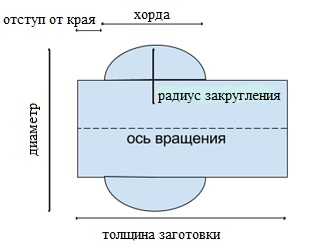
\includegraphics[width=0.5\linewidth]{cavity_scheme}
  \caption{Рисунок микрорезонатора ММШГ с параметрами для программы DAC DSL алмазного точения.}
  \label{cavity_scheme}
\end{figure}

Основными параметрами, влияющими на качество изготавливаемых микрорезонаторов ММШГ, являются скорость вращения шпинделя (\texttt{rpm}), линейная скорость точения (угловая скорость шпинделя умноженная на радиус резонатора), скорость движения резца (\texttt{feed rate}) и глубина захода (\texttt{depth of cut}). Опытным путем были определены следующие оптимальные параметры для точения кристаллов $MgF_2, CaF_2, BaF_2, LiNbO_3, LiTaO_3$:

\begin{itemize}
    \item \texttt{rpm}=400-1500;
    \item \texttt{feed\_rate}=2-3 мкм/оборот для предварительной обработки и <1-2 мкм/оборот для финального прохода;
    \item \texttt{depth\_of\_cut}=2-4 мкм для грубой обработки и 0.05-1 мкм для финального прохода.
\end{itemize}

Важнейшим фактором является охлаждение во время точения. Для этого на резец и резонатор распыляется охлаждающая жидкость, которая сразу же отсасывается в воздухозаборник вместе со срезанными стружками. В качестве охлаждения использовался изопропиловый спирт или Exxsol D100 – деароматизированная углеводородная жидкость. Жидкость не должна попадать внутрь шпинделя или линейных подач X,Y, а также должна быстро улетучиваться и не оставлять следов на кристалле. Без использования жидкости точение возможно, но с минимальной глубиной и скоростью подачи, при этом алмаз изнашивается значительно быстрее, а качество поверхности выточенного резонатора получается хуже.

После точения проводилась очистка микрорезонатора от кристаллической стружки с помощью полимерных салфеток, смоченных в метаноле. Сразу из-под резца получается добротность $10^5 - 10^6$. Дальнейшее увеличение добротности достигается последовательной ручной полировкой с помощью и алмазных суспензий с уменьшающимся размером зерна (2.5 - 1 - 0.5 - 0.25 - 0.1 – 0.03 мкм) по 10-15 мин каждой. Использовались алмазные суспензии Microdiamant OPW-20, вязкость 325 cP, pH = 8.0, концентрация алмазных зерен 15 карат/литр. Суспензии наносились на тканный текстиль AlliedHighTech. Преимуществом использования суспензий, нанесенных на мягкую текстильную подложку является возможность более плотного контакта с тороидальной поверхностью по сравнению с алмазными шкурками на полимерной пленке.

Важнейшим элементом процедуры является очистка резонатора после полировки каждой суспензией. Очистка проводилась теми же средствами, что и первичная очистка после точения, и длилась по 5 мин. При длительном нахождении микрорезонатора ММШГ в пыльном месте, может потребоваться повторная очистка для достижения максимальной добротности.

На рис. \ref{cavity_polished} приведены фотографии поверхностей микрорезонатора ММШГ сразу после точения изношенным резцом, фрагмент со сколом и после полировки алмазными суспензиями. Видно значительное улучшение качества поверхности.

\begin{figure}[ht]
  \begin{minipage}[ht]{0.32\linewidth}\centering
    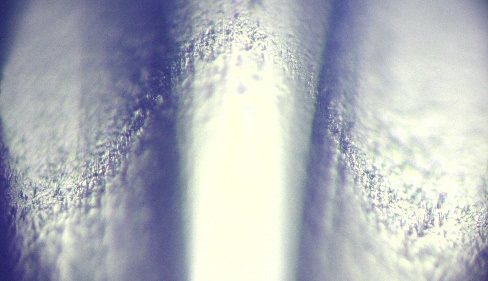
\includegraphics[width=1\linewidth]{cavity_unpolished}
  \end{minipage}
  \hfill
  \begin{minipage}[ht]{0.32\linewidth}\centering
    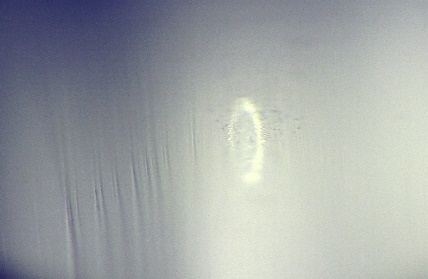
\includegraphics[width=1\linewidth]{cavity_polished_bad}
  \end{minipage}
  \hfill
  \begin{minipage}[ht]{0.32\linewidth}\centering
    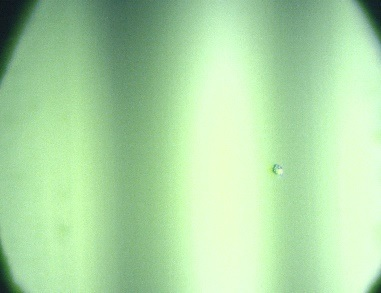
\includegraphics[width=1\linewidth]{cavity_polished_good}
  \end{minipage}
  \caption{Фрагмент поверхности резонатора с радиусом кривизны боковой поверхности 50 мкм (ширина выступа около 70 мкм). Слева сразу после точения изношенным резцом. Посередине фрагмент со сколом размером 20 на 50 мкм. Справа - после полировки алмазными суспензиями.}
  \label{cavity_polished}
\end{figure}

При увеличении глубины резки (depth of cut) до 6 мкм и более возможен хрупкий режим точения со сколами кристалла и повышенным износом резца. После очистки микрорезонатора проводится проверка качества получившейся поверхности в микроскоп для обнаружения возможных шероховатостей.

Так как обычный оптический микроскоп имеет дифракционный предел, дефекты малого размера в нем не видны, и на большом увеличении глубина резкости минимальна, видна очень малая область тороидальной боковой поверхности (не более 20 мкм), то контроль качества осуществлялся последовательным измерением добротности мод после полировки  алмазными суспензиями.

Дополнительно может быть произведен контроль качества боковой поверхности с помощью оптического профилометра Zygo NewView 7300. Результат измерения приведен на рис. \ref{cavity_profilometer}, измерены шероховатости размером 0.25 мкм.

\begin{figure}[ht]
\centering
  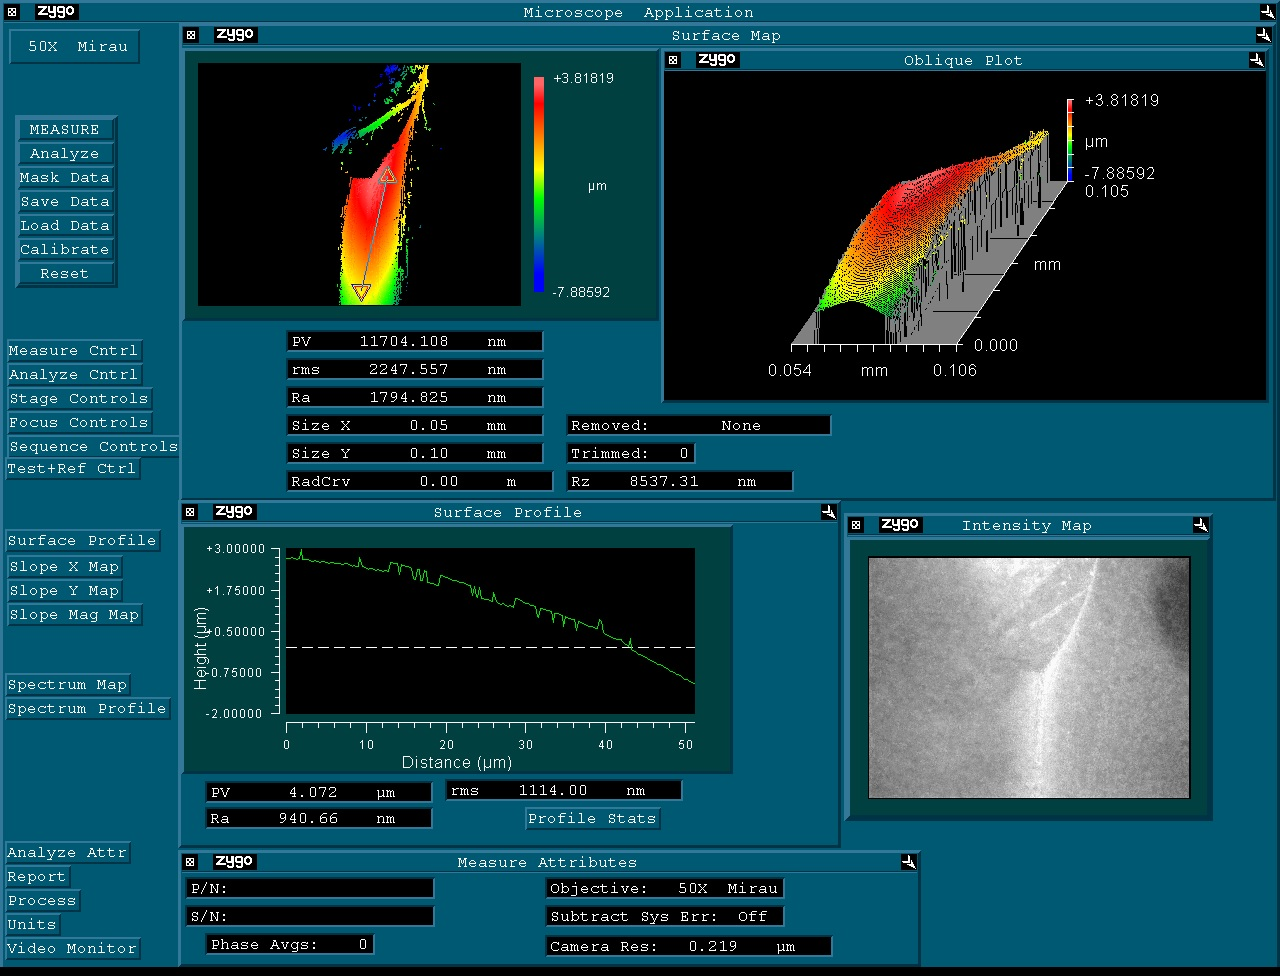
\includegraphics[width=0.5\linewidth]{cavity_profilometer}
  \caption{Измерение качества боковой поверхности с помощью оптического профилометра.}
  \label{cavity_profilometer}
\end{figure}

Достаточным условием для оценки качества поверхности является проверка добротности после полировки. К сожалению, при таком способе оценки качества поверхности можно упустить технические ошибки, возникающие при полировке, т.к. в данном случае о качестве можно судить только по косвенному признаку – добротности. Измерение добротности производилась следующими методами: калибровка частоты дается боковыми линиями фазовой модуляции сканирующего лазера, зная частоту модуляции, можно аппроксимировать лоренцевскую форму резонанса МШГ. Для измерения ширины линии резонанса меньше 500 кГц лучше использовать метод звона, при котором либо быстро выключается, либо быстро перестраивается по частоте лазер накачки и проводится прямое измерение времени звона оптического резонатора по затухающему сигналу фотодетектора. Для измерения сверхвысоких добротностей необходимо использовать мощность лазера меньше 1 мВт, чтобы избежать нелинейных уширений.

В таблице \ref{table_turning_params} представлены параметры точения, при которых получались наилучшие результаты для различных материалов.

\begin{table} [htbp]% Пример записи таблицы с номером, но без отображаемого наименования
	\centering
	\parbox{17cm}{% чтобы лучше смотрелось, подбирается самостоятельно
        %\captionsetup{format=tablenocaption}% должен стоять до самого caption
        \caption{Параметры алмазного точения резонаторов из различных кристаллических материалов}%
        \label{table_turning_params}%
    	\begin{tabular}{||c|c|c|c|c||}
\hline
\multicolumn{1}{|p{2cm}|}{\centering Материал} & \multicolumn{1}{|p{2cm}|}{\centering Скорость вращения шпинделя \\ обороты в мин} & \multicolumn{1}{|p{2cm}|}{\centering Скорость движения резца \\ мкм/оборот} & \multicolumn{1}{|p{2cm}|}{\centering Глубина захода резки \\ мкм} & \multicolumn{1}{|p{2cm}|}{\centering Охлаждающая \\ жидкость}\\
%Материал & Скорость вращения шпинделя, обороты в мин & Скорость движения резца, мкм/оборот & Глубина захода резки, мкм & Охлаждающая жидкость\\
\hline
$MgF_2$ & 400-1500 & 0.25-1 & 0.05-1 & да/нет \\
\hline
$BaF_2$ & 1000-2500 & 1-2.5 & 0.5-2 & нет \\
\hline
$CaF_2$ & 700-2500 & 1-2 & 1 & да/нет \\
\hline
$LiNbO_3$ & 900-1500 & 1-2.5 & 1-4 & нет \\
\hline
$LiTaO_3$ & 900 & 1-2 & 1-2 & нет \\
\hline
$Si$ & 500 & 1 & 0.5-1 & да \\
\hline
$TGG$ & 700 & 1 & 0.5-1 & нет \\
\hline
\end{tabular}

	}
\end{table}

\subsection{Практические замечания по изготовлению кристаллических микрорезонаторов}

Предобработка - раскол кристаллических пластин заготовок, при этом возможно образование напряжений внутри кусочков кристаллов. Мягкие материалы $BaF_2, CaF_2$ раскалываются на неконтролируемые куски при любой толщине заготовки. Распил алмазной пилой позволяет этого избежать. Однако для заготовок толщиной 100-200 мкм возможны внутренние трещины из-за неровности наклейки на подставку для распила. Необходимо использовать тонкие диски пилы с алмазным напылением. Выпиливание цилиндрических заготовок трубчатым сверлом малоэффективно, т.к. большая часть материала уходит в стружку, и из-за больших биений сверла вероятно появление больших сколов.

Дизайн подставки \ref{cavity_scheme_big} диктуется размером цанги станка и удобством крепления в экспериментальных установках. Материал подставки латунь выбран из-за достаточно высокой теплопроводности для улучшения активной термостабилизации. Все кристаллические материалы для генерации оптических гребенок имели z-cut, т.ч. оптическая ось z совпадала с осью цилиндра.

Отжиг кристаллов для устранения внутренних дефектов проводился, но без прямого измерения улучшения добротности до и после, т.к. клей не позволяет нагревать до 700-800С наклееный на подставку резонатор, а в случае переклейки резонатора вероятность загрязнения велика, и будет требоваться новая переполировка. При попытке отжига наклеенного резонатора из $BaF_2$ при 400С в кристалле возникло большое количество внутренних трещин.

Алмазное точение SPDT возможно в широком диапазоне параметров при использовании нового неизношенного резца. Качество поверхности фторида магния при этом высокое, т.ч. добротность резонатора может достигать $10^6$ (пример выступа резонатора с такой добротностью дан на рис. \ref{protrusion_unpolished}), что соответствует типичным значениям добротности в интегральных оптических резонаторах из $SiN$.

\begin{figure}[ht]
\centering
  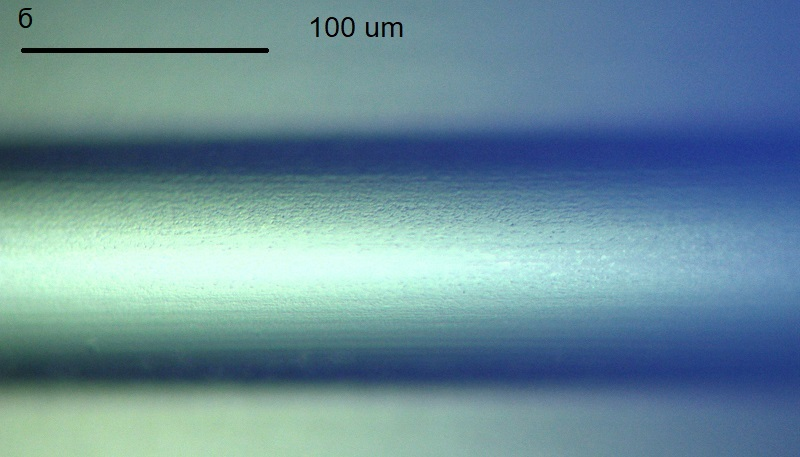
\includegraphics[width=0.5\linewidth]{protrusion_unpolished}
  \caption{Фотография поверхности резонатора из $MgF_2$ сразу после точения, в котором достигается добротность $10^6$ на 1550 нм.}
  \label{protrusion_unpolished}
\end{figure}

Основной недостаток метода алмазного точения - быстрый износ алмазного резца. На практике износ резца наступает за 100 м точения, что соответствует изготовлению 3 резонаторов. Далее качество получаемой поверхности заметно ухудшается и никакими более щадящими параметрами точения улучшить его нельзя. Изношенным резцом возможно точение твердых материалов $MgF_2$, но более мягкие $BaF_2, LiF$ могут давать сколы размерами в несколько сот микрон, недоступными для устранения полировкой \ref{cavity_damage}. Наиболее практично использовать для изготовления цилиндров заданного диаметра изношенный резец, а далее снимать финальный слой толщиной 10 мкм с помощью чистового неизношенного резца. Важно при этом регулярно проводить перекалибровку относительного положения изношенного и чистового резцов, т.к. сколы края алмаза могут достигать 10 мкм \ref{tool_damage}.

\begin{figure}[ht]
  \begin{minipage}[ht]{0.49\linewidth}\centering
    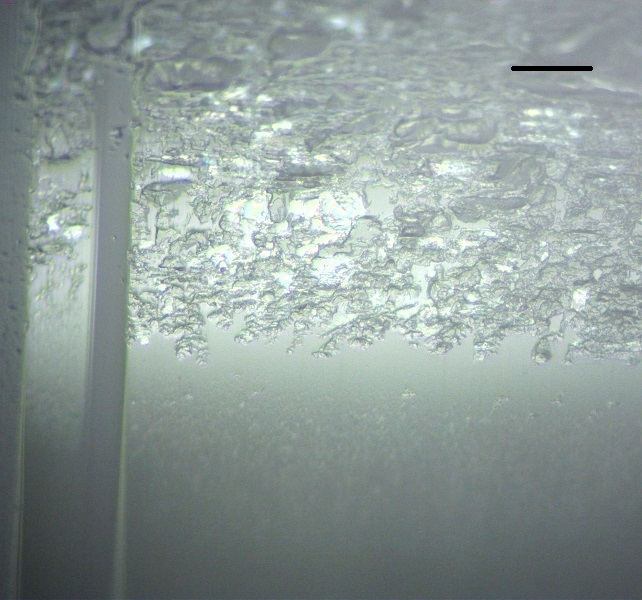
\includegraphics[width=1\linewidth]{cavity_damage}
  \end{minipage}
  \hfill
  \begin{minipage}[ht]{0.49\linewidth}\centering
    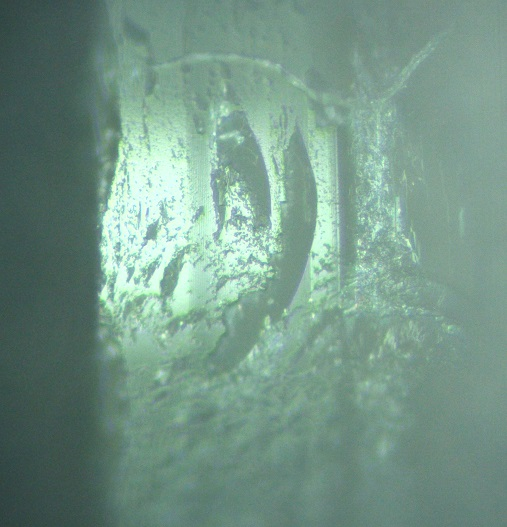
\includegraphics[width=1\linewidth]{cavity_damage_baf2}
  \end{minipage}
  \caption{Слева фрагмент поверхности резонатора из $MgF_2$ после точения при неоптимальных параметрах, видны секторы хорошего и плохого качества поверхности, соответствующие точению различных кристаллических срезов, такие дефекты можно убрать полировкой без сохранения геометрии резонатора. Справа фрагмент поверхности резонатора из $BaF_2$ после точения изношенным резцом, видны глубокие сколы, которые нельзя убрать полировкой.}
  \label{cavity_damage}
\end{figure}

\begin{figure}[ht]
\centering
  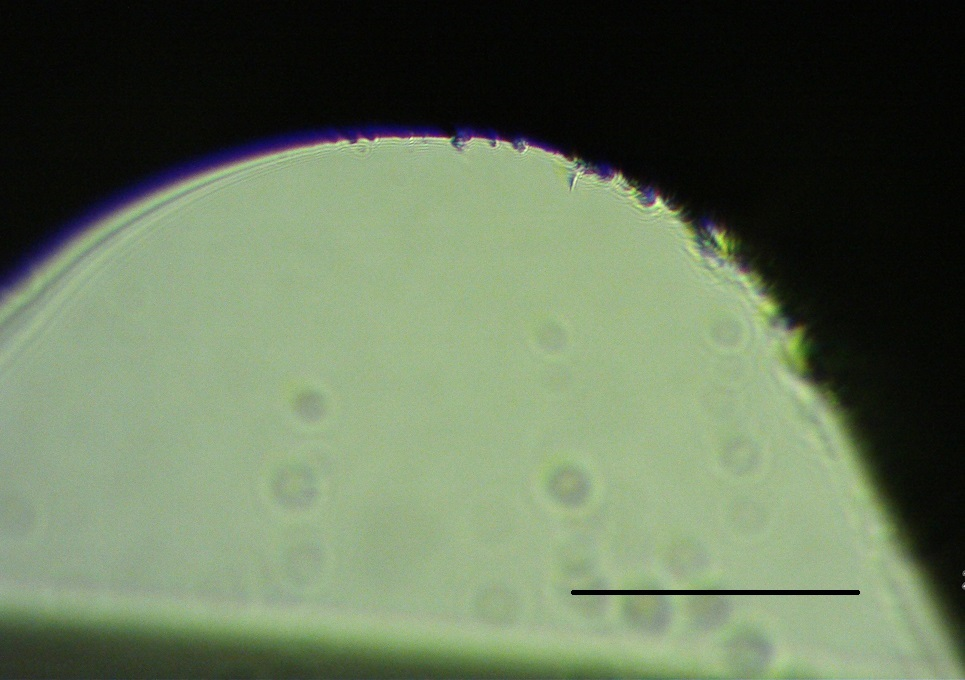
\includegraphics[width=0.5\linewidth]{tool_damage}
  \caption{Рабочий край изношенного алмазного резца с радиусом кривизны 500 мкм и наклоном рабочей грани -25, видны сколы по краю характерным размером 10 мкм. При дальнейшем использовании резца возможно образование скола алмаза по прямой линии, таким резцом можно грубо вытачивать цилиндры заданного диаметра.}
  \label{tool_damage}
\end{figure}

В литературе по точению основными методами борьбы с износом являются более щадящие параметры точения (уменьшение глубины резки и действующей силы, пропорциональной скорости вращения) и использовании охлаждающей жидкости. Важно понимать, что при использовании охлаждающей жидкости меняется режим точения, и следует заново подбирать оптимальные параметры. Уменьшение же глубины резки приводит к пропорциональному росту времени точения. Охлаждающая жидкость при изготовлении большинства резонаторов из $MgF_2$ не применялась, т.к. нет удобной системы вентиляции, и ее расход велик, т.ч. бака может не хватать на типичное точение в 6-10 часов, также заводская жидкость содержала маслянистые фракции, которые могут повредить шпиндель на воздушных подшипниках.

Полировка при хорошей центровке микрорезонатора возможна не только последовательным уменьшением зерна суспензии, но и при грубой полировке зерном 2.5-4 мкм для удалений сколов с характерными размерами 5-15 мкм, далее зерном 0.5 мкм и сразу 0.1 мкм для финальной полировки. Стандартное правило - удаление материала в 3-4 кратном размере диаметра зерна. Таким способом повторяемо достигается добротность $5*10^8$ на длине волны $1550 нм$ в кристаллах $MgF_2$ из заготовки VUV качества материала \ref{ringdown}.

\begin{figure}[ht]
\centering
  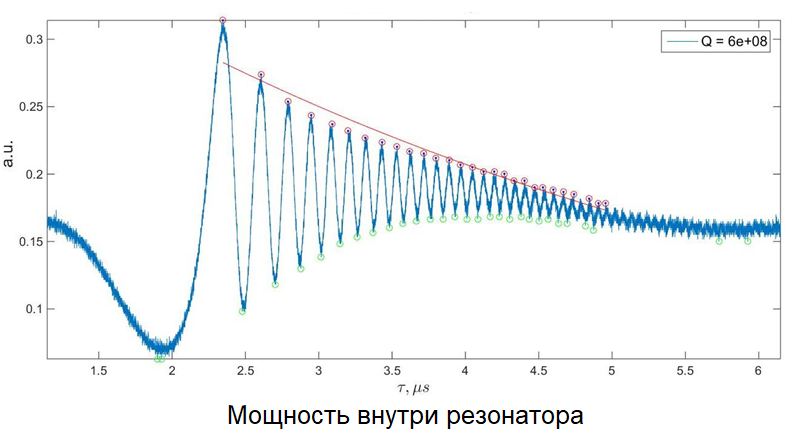
\includegraphics[width=0.5\linewidth]{ringdown1billion}
  \caption{Определение добротности резонатора из $MgF_2$ прямым измерением времени звона оптического резонатора. Соответствующее значение добротности $2*10^9$}
  \label{ringdown}
\end{figure}


Изготовление прямоугольных микровыступов даже новыми острыми резцами не удалось для диаметров резонатора больше 4 мм для $MgF_2$ и получилось для диаметров около 1 мм \ref{protrsuion_rect}. Этот резонатор далее детально не изучался.

\begin{figure}[ht]
\centering
  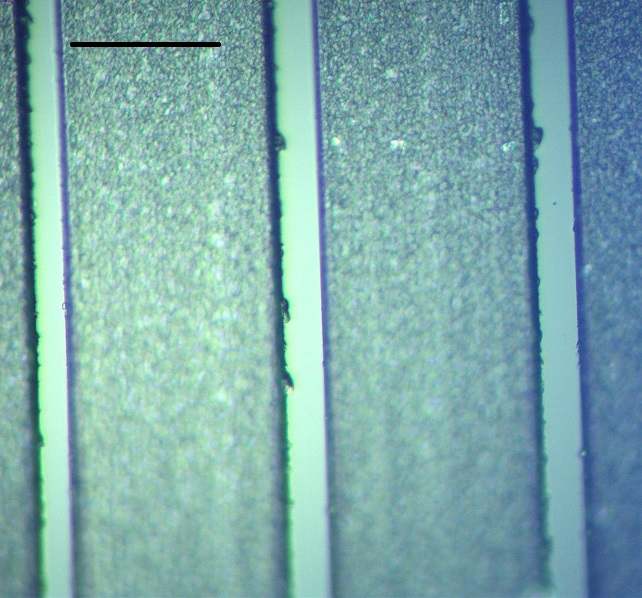
\includegraphics[width=0.5\linewidth]{protrsuion_rect}
  \caption{Фрагмент поверхности резонатора с прямоугольными выступами размером 5 на 15, 20, 25 мкм для контроля ДГС резонатора. Показано качество поверхности до полировки, видны сколы по 5 мкм на выступе из-за износа острого резца.}
  \label{protrsuion_rect}
\end{figure}

\section{Экспериментальное наблюдение оптических частотных гребенок и солитонов в резонаторах из $MgF_2$}


\subsection{Экспериментальная установка и результаты генерации солитонов}

Для генерации оптических гребенок и солитонов в кристаллических микрорезонаторах использовалась следующая экспериментальная схема \ref{Setup_CoProp}. Волоконный узкополосный перестраиваемый лазер непрерывной мощности (Koheras Adjustik) подается на фазовый или амплитудный модулятор, далее сигнал усиливается эрбиевым волоконным усилителем (Koheras), ASE шумы подавляются узкополосным пропускающим оптическим фильтром (Dicon). Далее свет проходит через волоконный контроллер поляризации (FPC) и заводится в резонатор через элемент связи - растянутое волокно, через него же свет из резонаторы выводится. Волоконный Брэгговский фильтр (AOS) используется для подавления мощной линий накачки, далее оптический сигнал подается на оптический спектроанализатор (OSA) и быстрый фотодетектор, электрический сигнал с которого измеряется осциллографом и спектроанализатором.

Растянутое волокно изготавливалось методом травления в плавиковой кислоте: зачищенное от пластика волокно диаметром 125 мкм помещалось в 100 мкл каплю 40 процентной плавиковой кислоты на 15 мин, далее в буферный раствор 18 процентной кислоты, в котором волокно травилось около 30 мин. Контроль толщины осуществлялся по сигналу пропускания через волокно, наблюдалась характерная осцилляционная картина, травление прекращалось сразу после исчезновения осцилляций. Таким методом были получены волокна с конической перетяжкой и диаметром перетяжки от 3 до 8 мкм. Растянутые волокна выдерживали мощность до 300 мВт.

\begin{figure}[ht]
\centering
  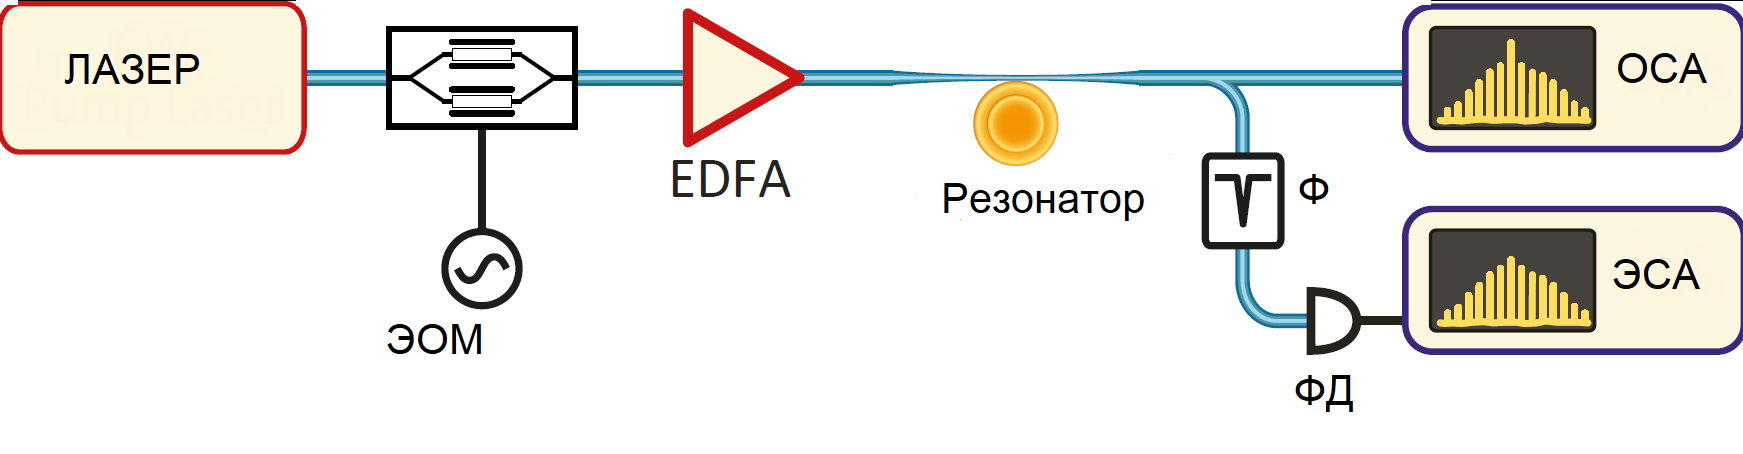
\includegraphics[width=0.4\linewidth]{Setup_CoProp}
  \caption{Cхема экспериментальной установки для генерации оптических гребенок и солитонов.}
  \label{Setup_CoProp}
\end{figure}

Для настройки на шумную гребенку \ref{step_schematics} достаточно медленно перестроить частоту лазера из области синей отстройки в область верхней ветви керровских частотных гребенок. Пример генерации шумных оптических гребенок и широкого сигнала биений на частоте ОСД дан на рис. \ref{wide_comb_93GHz,noisy12}.

\begin{figure}[ht]
\centering
  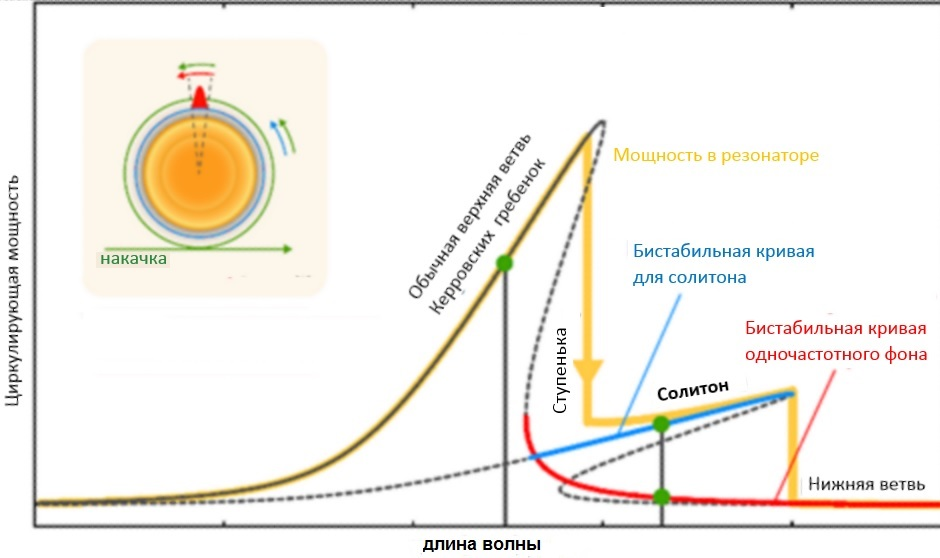
\includegraphics[width=0.4\linewidth]{step_schematics}
  \caption{Cхематичное изображение нелинейного резонанса с солитонной ступенькой}
  \label{step_schematics}
\end{figure}

\begin{figure}[ht]
\centering
  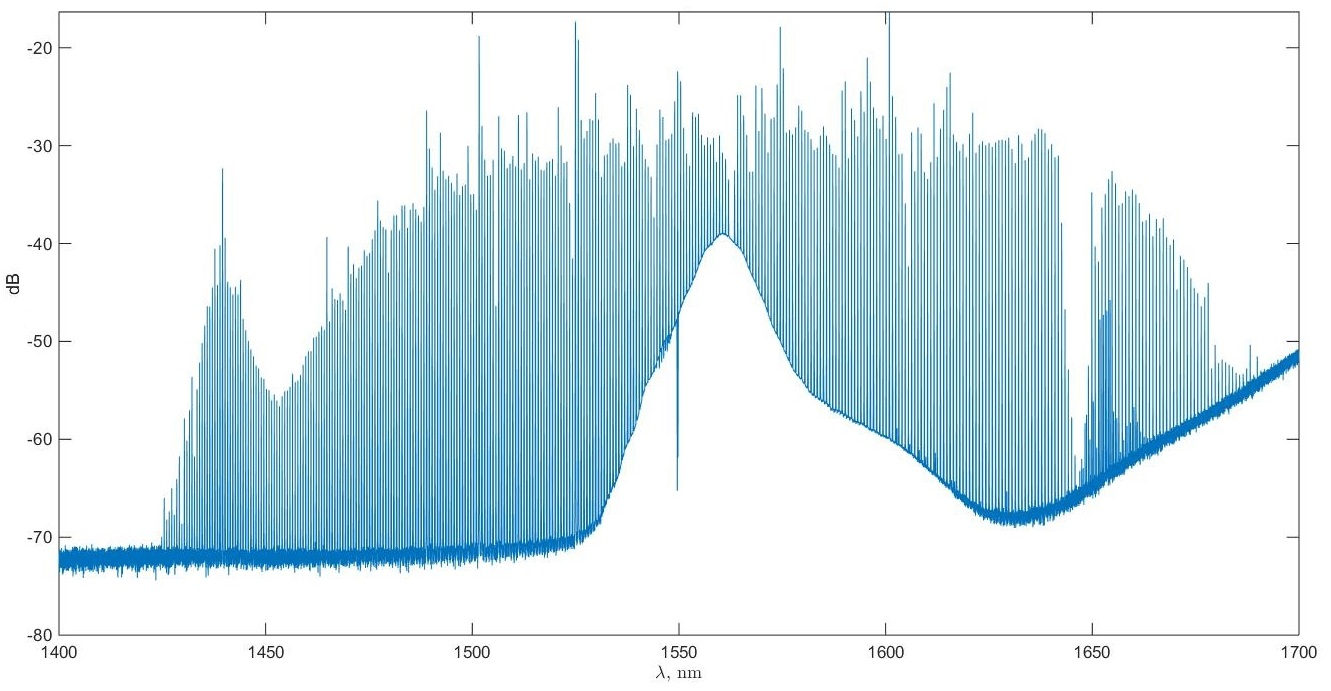
\includegraphics[width=0.4\linewidth]{wide_comb_93GHz}
  \caption{Оптический спектр широкой оптической гребенки в шумном режиме с ОСД около 93 ГГц, полученный в резонаторе диаметром 0.75 мм и радиусом кривизны 150 мкм.}
  \label{wide_comb_93GHz}
\end{figure}

\begin{figure}[ht]
  \begin{minipage}[ht]{0.49\linewidth}\centering
    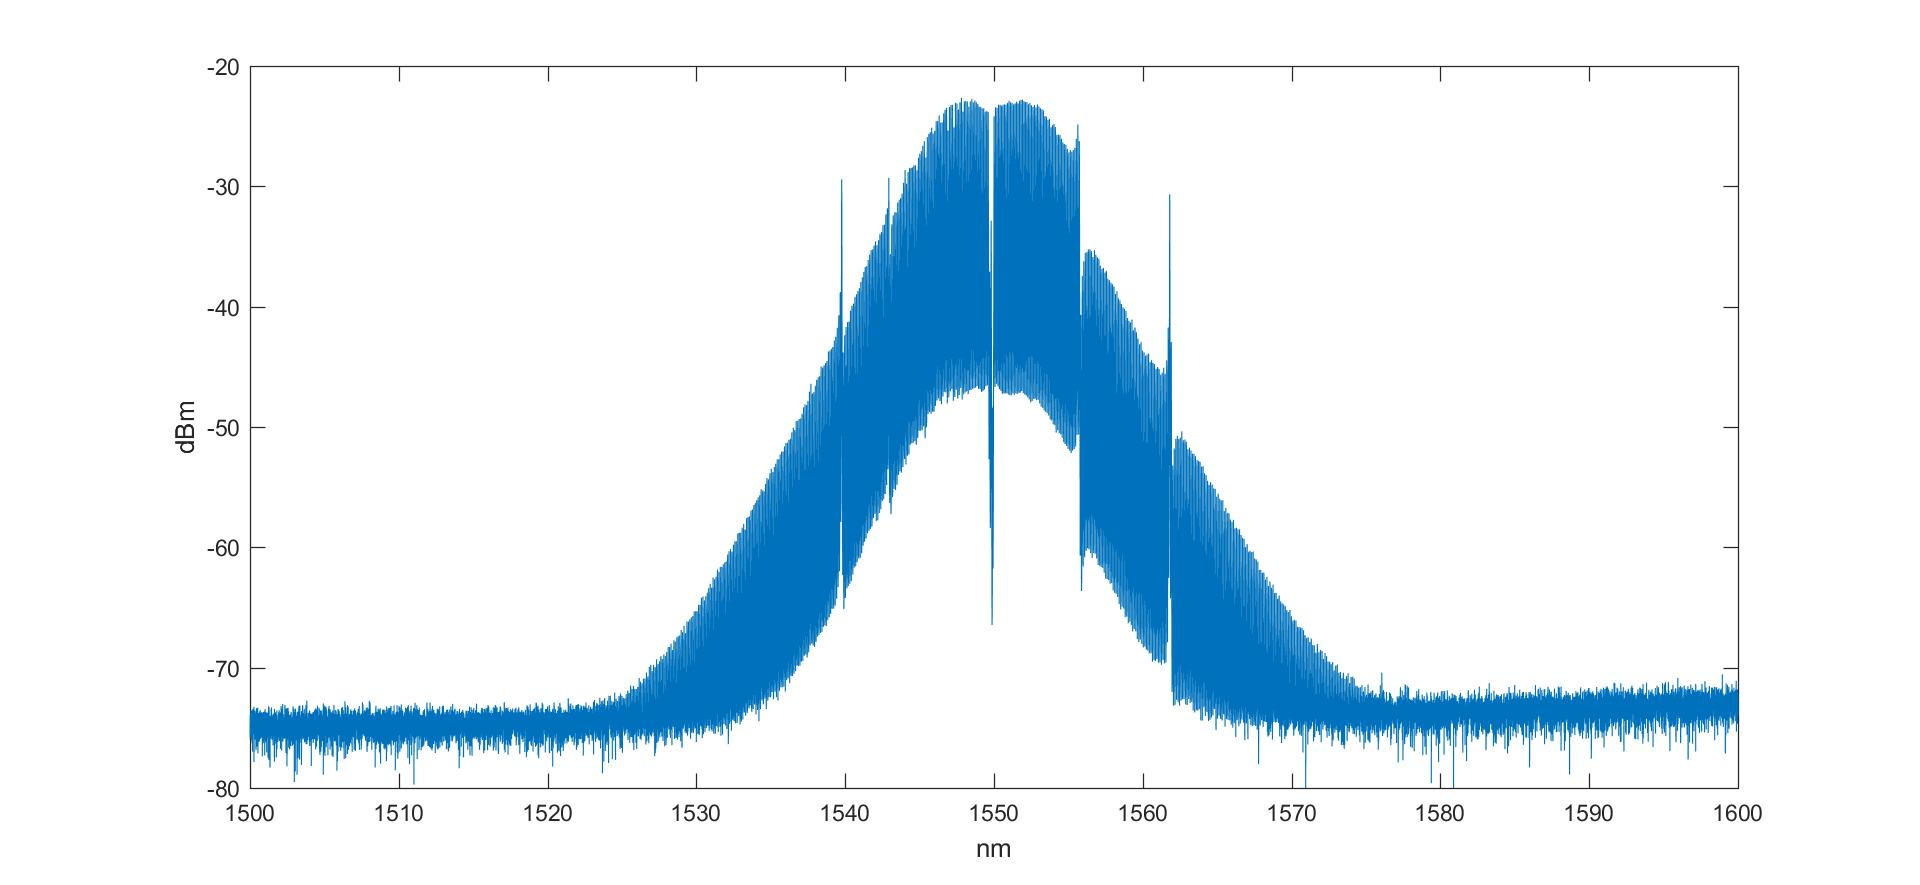
\includegraphics[width=1\linewidth]{noisy12}
  \end{minipage}
  \hfill
  \begin{minipage}[ht]{0.49\linewidth}\centering
    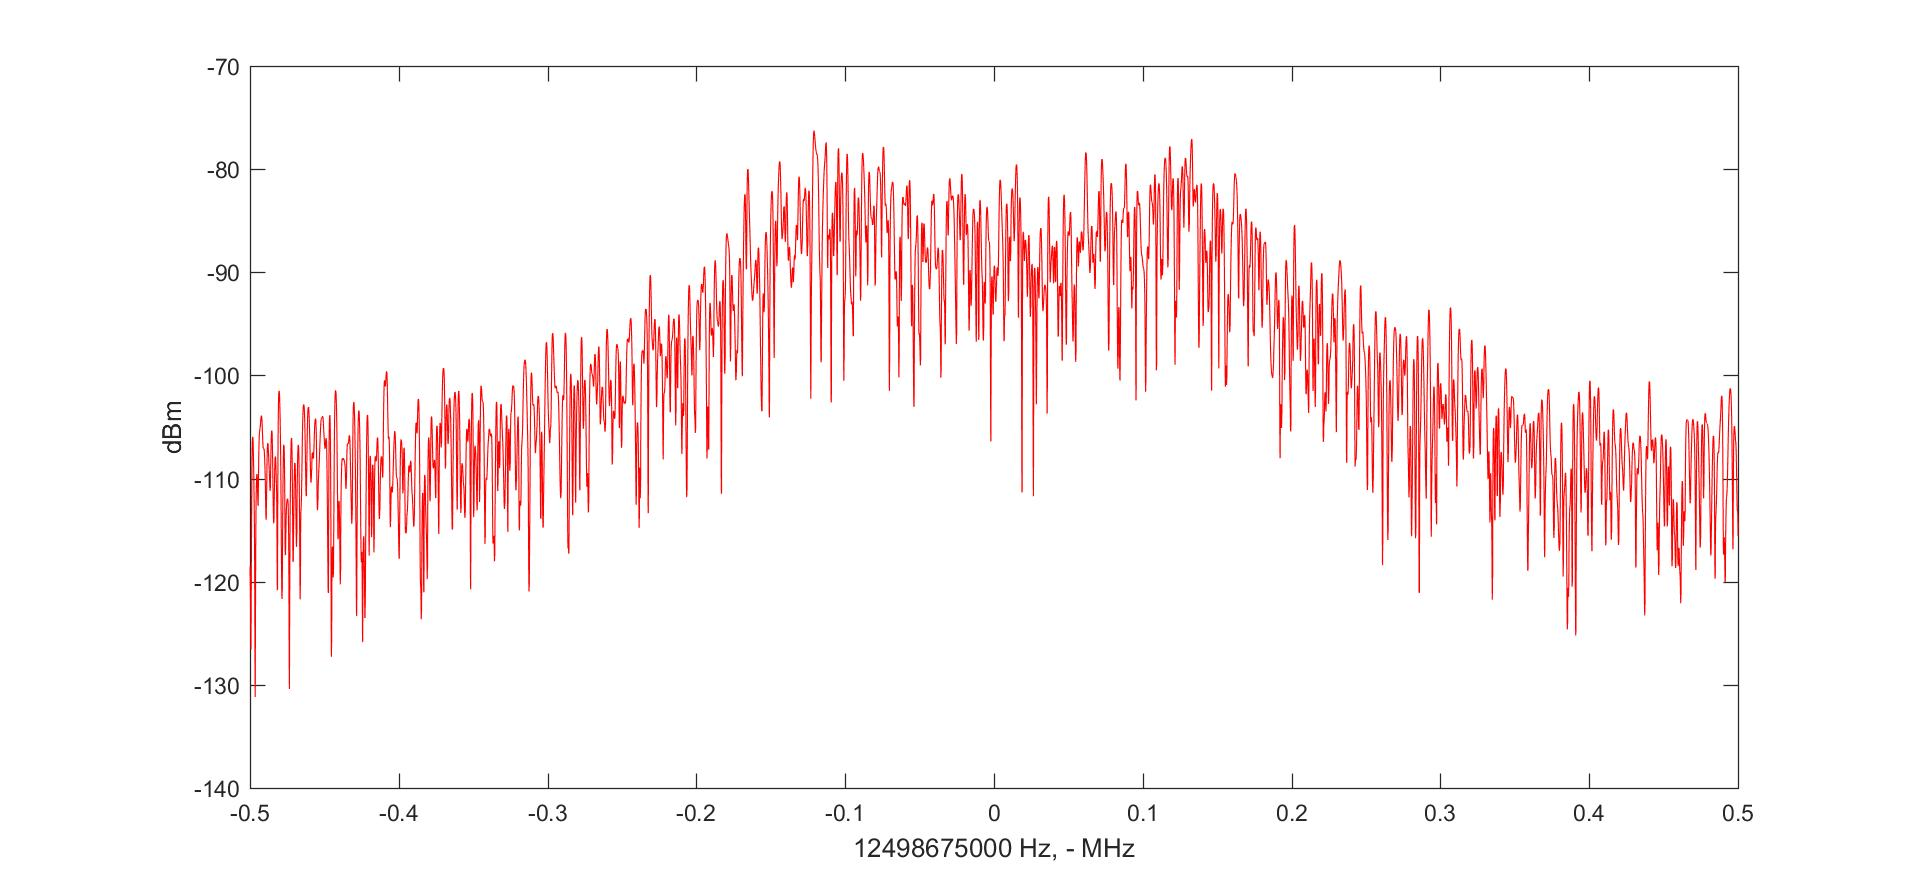
\includegraphics[width=1\linewidth]{noisy12_beatnote.jpg}
  \end{minipage}
  \caption{Слева оптический спектр оптической гребенки в шумном режиме. Справа соответствующий сигнал биений на частоте ОСД 12.48 ГГц.}
  \label{noisy12}
\end{figure}

Конический профиль растянутого волокна позволяет удобно изменять связь с модами резонатора путем его перемещения вверх, вниз и вдоль выступа резонатора и достигать оптимального положения, при котором солитонная ступенька наиболее широкая и мощная.

Для достижения солитонного режима требуется быстрая перестройка лазера, т.ч. тепловой нагрев и сдвиг моды резонатора не привел к выходу частоты лазера накачки из области существования солитона \ref{step_schematics}. Для этого подается однократное пилообразное напряжение на пьезоконтроллер частоты лазера, т.ч. окончание быстрой перестройки частоты совпало с центром области существования солитона. Для ступенек шириной более 6 МГц при мощности накачки до 120 мВт этого метода достаточно для повторяемого достижения солитонного режима в разных резонаторах \ref{soliton_12GHz,clean_27GHz_single_soliton}. В ходе работы были получены солитоны только в резонаторах из материала $MgF_2$, т.к. в нем при нагреве мощным лазером накачки терморефрактивный эффект компенсирует сдвиг собственных частот, вызванный тепловым расширением (в материалах $CaF_2$,$BaF_2$ при накачке мощным лазером возникают сильные термооптические осцилляции и достижение стационарного режима оптических гребенок затруднительно). В ходе работы были получены солитоны с частотами повторений от 8.5 ГГц до 27 ГГц. В резонаторах малого диаметра тепловая нелинейность преобладает и ширина солитонных ступенек меньше 1 МГц, что требует дополнительных методов настройки.

\begin{figure}[ht]
  \begin{minipage}[ht]{0.49\linewidth}\centering
    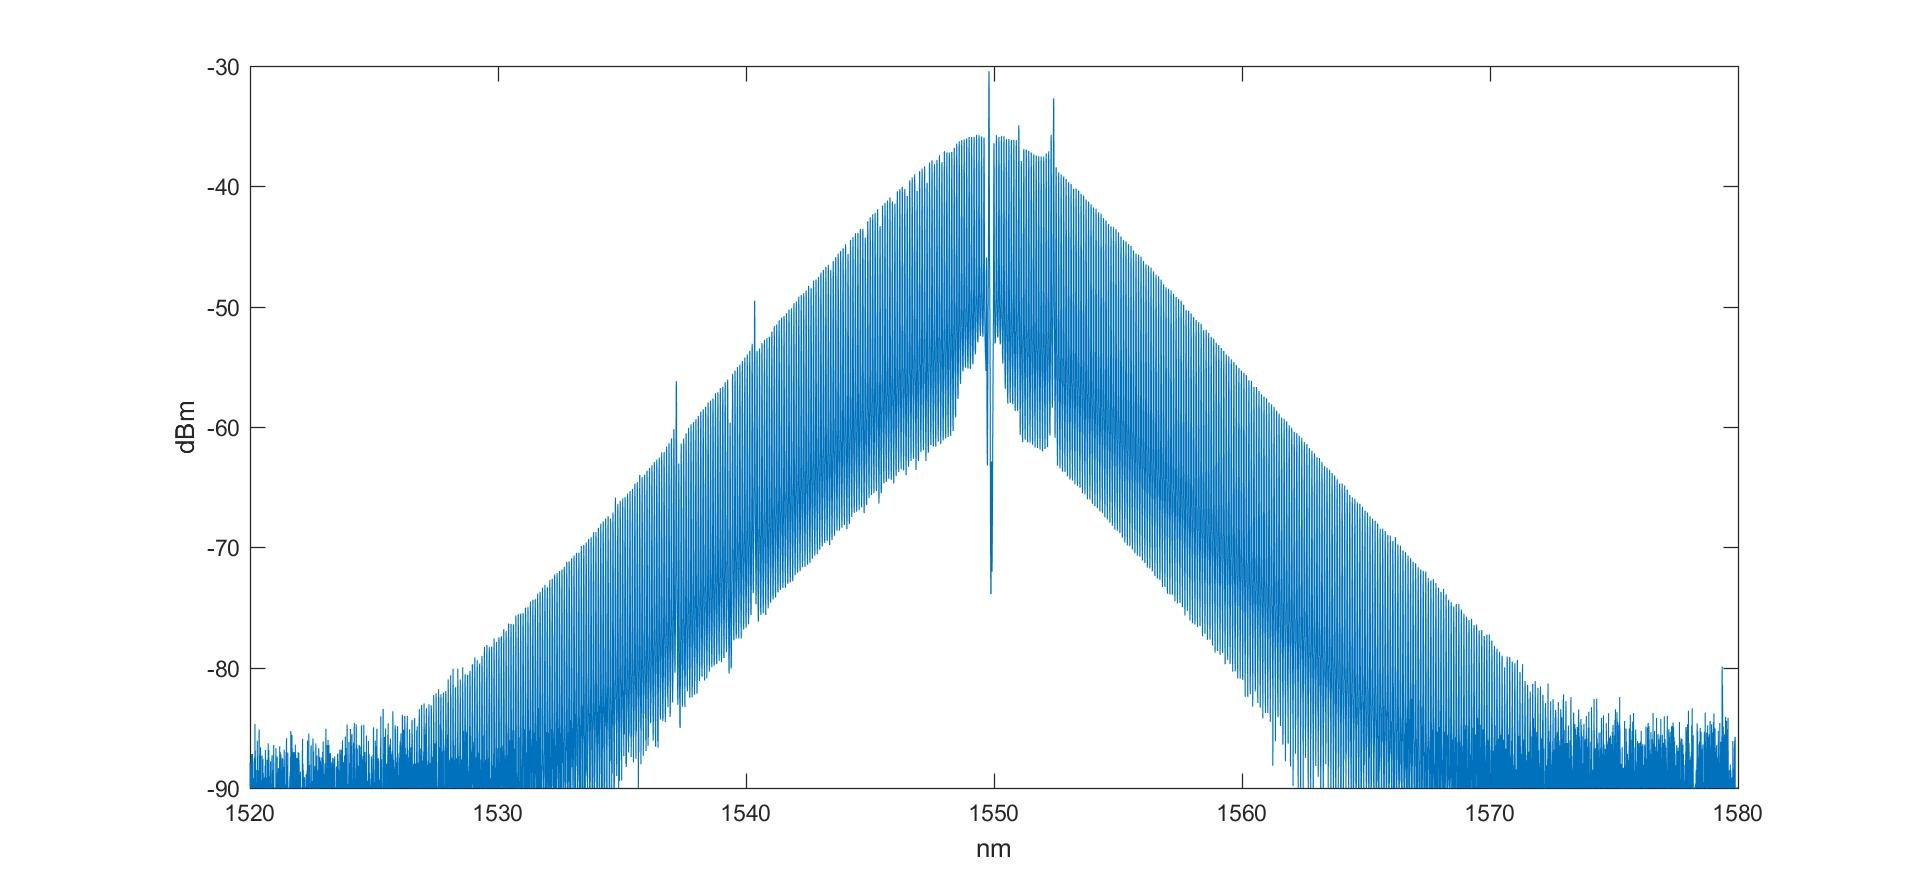
\includegraphics[width=1\linewidth]{soliton_12GHz}
  \end{minipage}
  \hfill
  \begin{minipage}[ht]{0.49\linewidth}\centering
    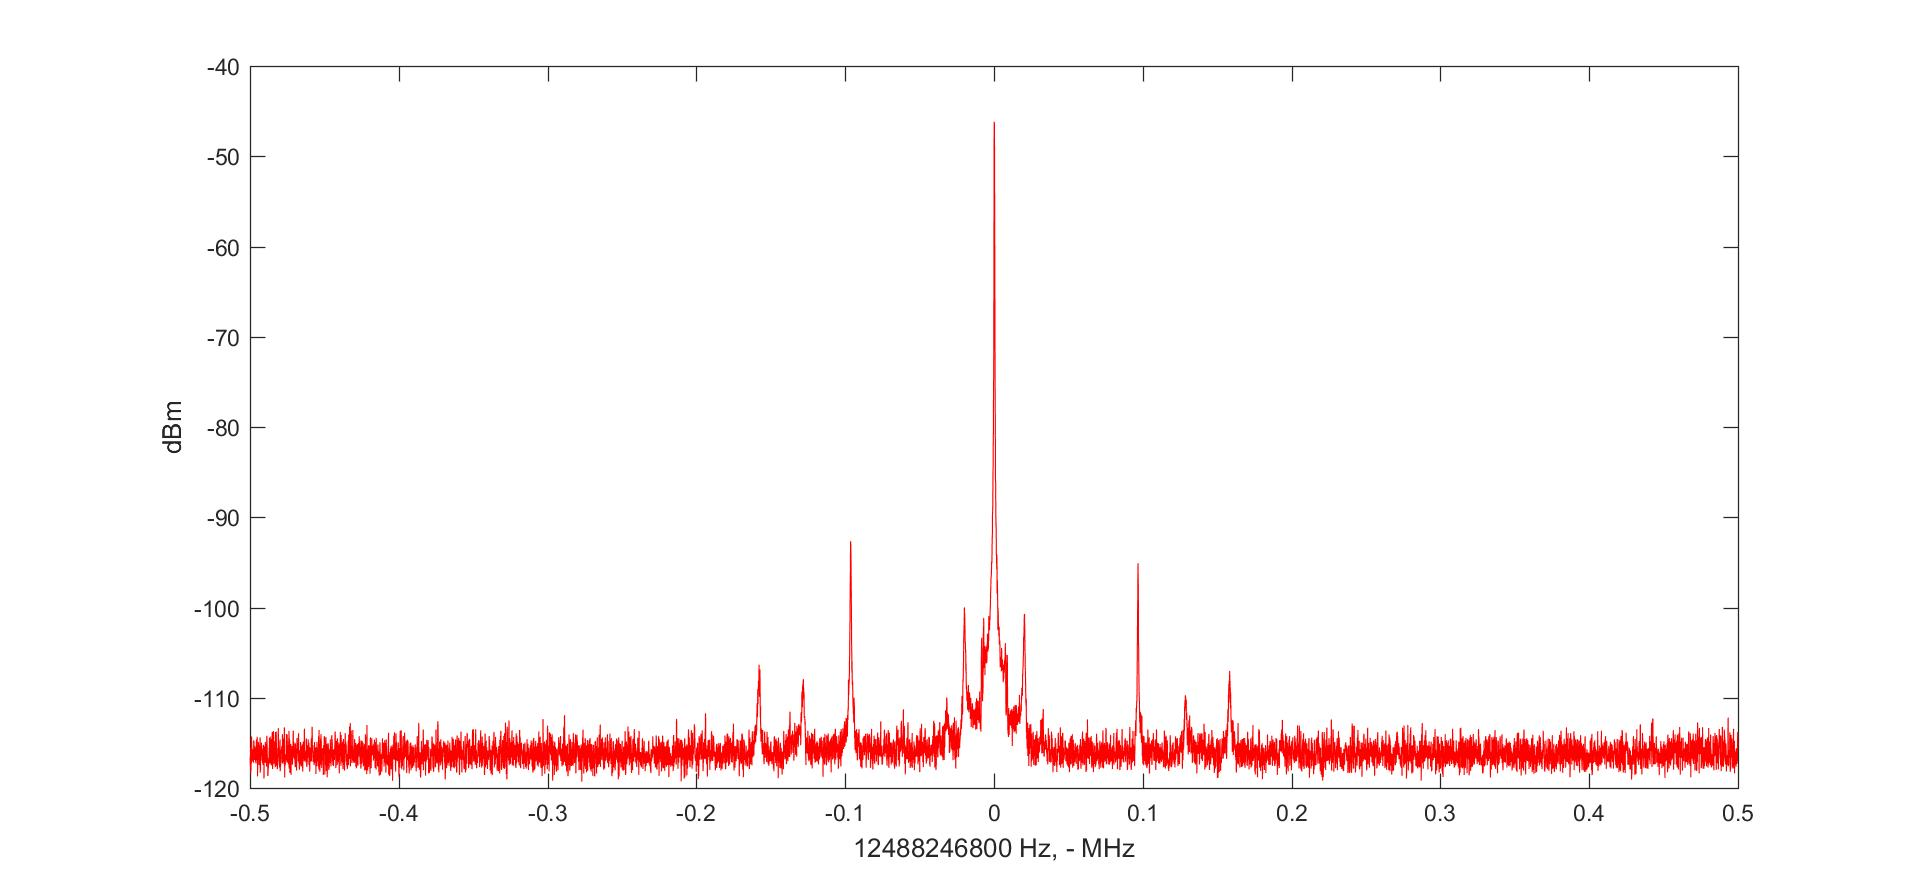
\includegraphics[width=1\linewidth]{soliton12_beatnote.jpg}
  \end{minipage}
  \caption{Слева оптический спектр оптической гребенки в односолитонном режиме. Справа соответствующий узкий сигнал биений на частоте повторения солитона 12.48 ГГц}
  \label{soliton_12GHz}
\end{figure}


\begin{figure}[ht]
\centering
  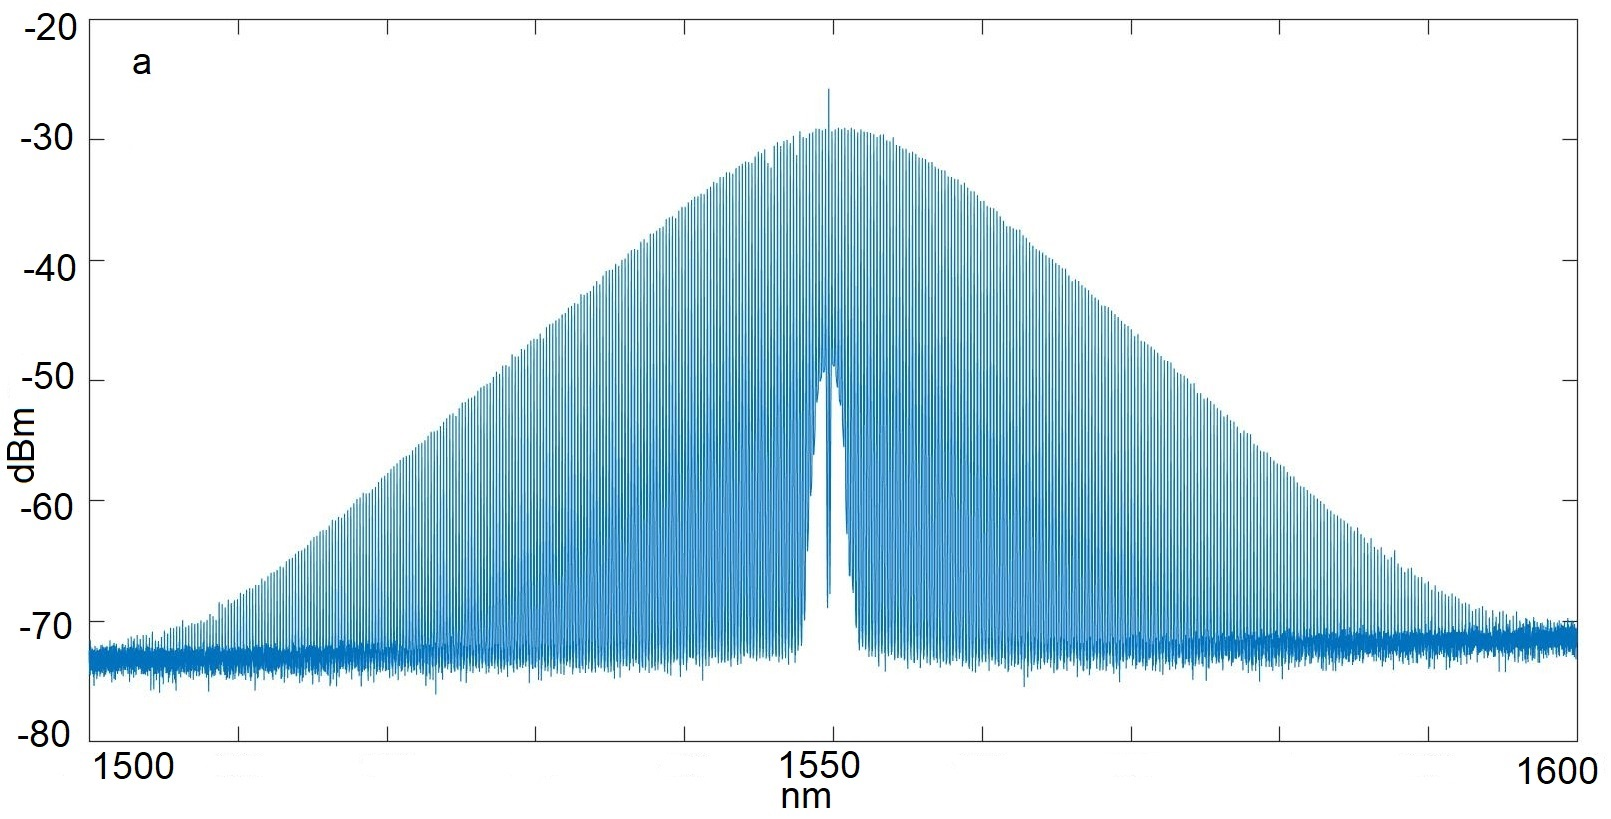
\includegraphics[width=0.5\linewidth]{clean_27GHz_single_soliton}
  \caption{Оптический спектр односолитонного режима с ОСД около 27 ГГц, полученный в резонаторе диаметром 2.4 мм и радиусом кривизны 80 мкм. Регулируя положение элемента связи (оптического волокна) с резонатором возможно добиться спектра с минимальным количеством пересечений мод}
  \label{clean_27GHz_single_soliton}
\end{figure}

Для контроля текущего значения отстройки лазера от частоты холодного резонанса лазер накачки фазово модулировался сигналом, подающимся с панорамного индикатора (RIGOL Network Analyser), далее сигнал пропускания системы с фотодетектора подавался на панораму и наблюдались 2 пика \cite{Karpov2017}, один из которых соответствовал текущей отстройке лазера от резонанса МШГ, другой пик говорил о наличии и количестве солитонов. Таким образом можно вручную подстраивать частоту лазера для стабилизации солитона в текущем многосолитонном и односолитонном режиме.

Без активной стабилизации частоты лазера время жизни солитона составляло от секунды до 20 мин, за это время лазер накачки уходил из области существования солитона. Для долгосрочной стабилизации была использована схема PDH (Pound-Drever-Hall), в котором на лазер накачки подавалась фазовая модуляция на заданной частоте, отклик системы в форме сигнала пропускания подавался на фазовой детектор вместе с исходным сигналом модуляции, сдвинуты по фазе. Получившийся сигнал ошибки подавался на PID контроллер, усиливался и подавался на пьезоконтроллер частоты лазера. Подбирая точку стабилизации на солитонной ступеньке путем изменения частоты модуляции и фазы опорного сигнала для фазового детектора, можно получить уединенный крутой склон в сигнале ошибке. Далее эмпирически подбирая параметры усиления PID контроллера, можно существенно облегчить процесс настройки на солитон - так при включенной системе обратной связи настройка на солитон путем быстрой перестройки частоты лазера дает положительный результат почти всегда. После настройки на солитонный режим включается интегратор PID на полный диапазон частот, и солитон стабилизируется на несколько часов. Недостатком схемы PDH для данной задачи является отсутствие возможности перестраивать отстройку без выключения солитонного режима. Также использовалась схема активной стабилизации температуры резонатора с помощью элемента Пельтье, диодного сенсора температуры и PID контроллера.

%\subsection{Метод стабилизации частоты повторения солитонов с помощью амплитудной модуляции лазера накачки}
%амплитудная модуляция на кратных фср частотах приводит к узкой области захватывания частоты повторения солитонов

\subsection{Методы достижения односолитонного режима}

В литературе было предложено несколько методов детерминированного достижения односолитонного режима в оптических микрорезонаторах. Первый метод предполагает одновременную перестройку частоты лазера накачки и изменение его мощности для избежания хаотического режима гребенки \cite{Jaramillo2015}. Другим способом является не перестройка частоты лазера, а сдвиг частоты резонанса МШГ путем изменения его температуры \cite{Joshi2016} или контроля времени жизни свободных носителей (для интегральных резонаторов) \cite{Yu2016}.

Рассмотрим случай \cite{Lobanov2016} фазовой $f(t)=F e^{i\varepsilon\sin\Omega t}$ и амплитудной $f(t)=F(1+\varepsilon\cos\Omega t)$  модуляции с частотой $\Omega$ и глубиной модуляции $\varepsilon$. Моделировалась система нелинейных связанных уравнений \ref{set_am}. Тепловые эффекты не рассматривались. В численных симуляциях не рассматривались частотная зависимость нелинейности, потерь и пересечения мод, взаимодействия между модами. Предполагая, что частота модуляции близка к ОСД резонатора:

\begin{equation}
\frac{\partial a_\mu}{\partial \tau}=-(1+\zeta_\mu)a_\mu+i\sum_{\mu',\mu^{''}}a_{\mu^{'}} a_{\mu^{''}} a^{*}_{\mu^{'}+\mu^{''}-\mu}+f_{\mu}\exp(i\mu\Delta\tau).
\end{equation}

Где обозначения соответствуют принятым в этой работе и $f_\mu=F J_\mu(\varepsilon)$ для фазовой модуляции и $f_{-1,0,1}=F[\varepsilon/2,1,\varepsilon/2]$,  $f_{\mu \neq -1,0,1}=0$ для амплитудной модуляции и безразмерной величине накачки $F$. $J_\mu(\varepsilon)$ функция Бесселя порядка $\mu$, $\Delta=2(D_1-\Omega)/\kappa$ нормализованная отстройка от точного значения ОСД, $D_1$ соответствует $2\pi\times$FSR. Все номера мод $\mu$ определены относительно 0 моды накачки. Дисперсионный закон дается разложением $\omega_\mu=\omega_0+D_1\mu+\frac{1}{2}D_2\mu^2+...$ и пренебрегая дисперсией третьего и более высоких порядков, получаем выражение для нормализованной отстройки: $\zeta_\mu=2(\omega_0-\omega_p)/\kappa+(D_2/\kappa)\mu^2$. $D_2>0$ соответствует аномальной дисперсии. Моделировалось 525 мод. Для анализа вычислялась средняя мощность внутри резонатора $U=\sum_{\mu} \vert a_\mu\vert^2$ для разных занчений нормализованной отстройки $\zeta_0$ и соответствующий профиль поля в микрорезонаторе $\psi(\varphi)=\sum_{\mu} a_{\mu}\exp(i\mu\varphi)$.

Для возбуждения солитонов лазер накачки перестраивается линейно по частоте $\zeta_{0}(\tau)=\zeta_{0}(0)+\alpha\tau$ от эффективной синей отстройки $\zeta_0(0)<0$, через нулевую отстройку в эффективную красную область $\zeta_0\gg0$ для сканирования всей области существования солитона. Формирование солитонов дает характерные ступеньки в генерируемом свете. Если перестройку лазера остановить на частоте, лежащей на ступеньке, то солитонное состояние является стабильным во времени. Максимальная частота отстройки области существования солитона \cite{Herr2014} дается $\zeta_{0\text{max}}\sim {\pi^2 F^2}/{8}$. В симуляциях использовались следующие значения $F\approx 4.11$, $D_{2}/\kappa\approx {0.01}$ и $\zeta_{0\text{max}}\approx 20.8$

Для набора статистики проводилось по 100 симуляций для каждого набора параметров и строилось распределение вероятности количества генерируемых солитонов. Известно \cite{Herr2014, Karpov2016}, что в случае немодулированной накачки ($\varepsilon=0$) количество возбуждаемых солитонов может варьироваться от скана к скану. Это подтверждается и при численном моделировании рис. \ref{Mod4}(a)-\ref{Mod4}(b). Среднее количество возбуждаемых солитонов увеличивается с увеличением мощности накачки и уменьшении ДГС резонатора. При уменьшении скорости сканирования лазера более вероятными становятся малосолитонные режимы.

\begin{figure}[ht]
\centering
  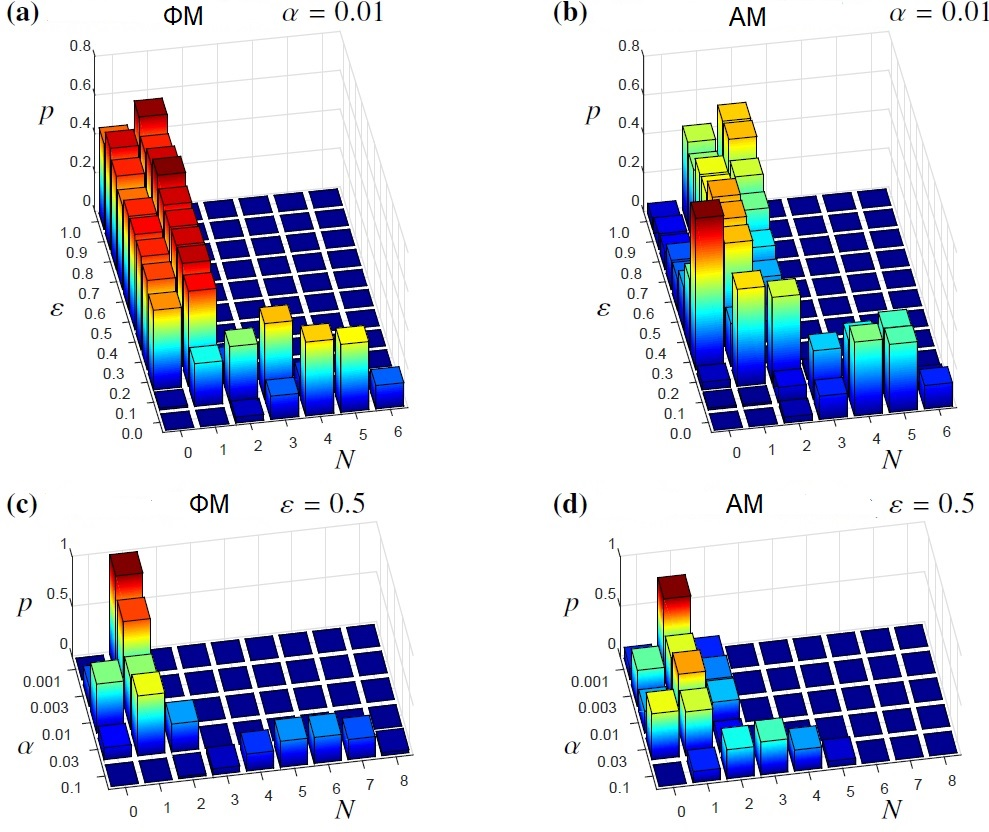
\includegraphics[width=0.85\linewidth]{Modulation4_s}
  \caption{Распределение вероятностей количества возбужденных солитонов от глубины модуляции $\varepsilon$ и скорости сканирования $\alpha$. Конечная отстройка $\zeta_0=18$ для фазовой и $\zeta_0=15$ для амплитудной модуляции. В обоих случаях $F\approx 4.11$, $100$ реализаций.}
  \label{Mod4}
\end{figure}

Статистика значительно изменяется при включении слабой резонансной модуляции ($\Delta=0$) на частоте 1 ОСД. Как показано на рис. \ref{Mod4}(a)-\ref{Mod4}(b), если глубина модуляции достаточно высокая ($\varepsilon> 0.2$), то более вероятными становятся состояния с меньшим количеством солитонов. Для фазовой модуляции возможны два равновероятных сценария - возбуждение односолитонного режима или отсутствие генерации солитонов вообще. Для амлитудной модуляции наиболее вероятные сценарии одно- или двухсолитонные состояния. Этот факт может быть объяснен взаимодействием солитонов: под действием фазовой модуляции солитоны внутри микрорезонатора двигаются к положению равновесия. Два солитона сталкиваются и уничтожаются, т.ч. суммарное число солитонов уменьшается на 2. Либо два солиотна сливаются в один с уменьшением общего числа на 1.

Важным фактором увеличивающем вероятность односолитонного режима является уменьшение скорости сканирования частоты лазера. При малых $\alpha$ для детерминированного достижения односолитонного режима требуется меньшая глубина модуляции. После остановки перестройки частоты лазера и достижения солитонного режима, возможно отключение модуляции с сохранением солитона, если глубина модуляции невелика.

При модуляции не строго на частоте 1 ОСД (Рис. \ref{Detuned}), а с неточностью $\Delta$, вероятность достижения односолитонного режима ниже и предложенный метод не так эффективен, что частично можно компенсировать увеличением глубины модуляции.

\begin{figure}[ht]
\centering
  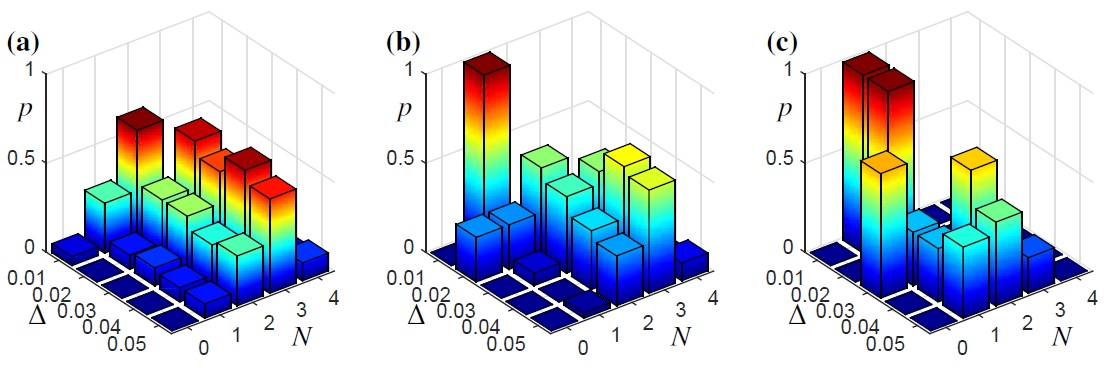
\includegraphics[width=0.85\linewidth]{detuned}
  \caption{Распределение вероятностей количества возбужденных солитонов при фазовой модуляции для различных значений неточности $ \Delta$  и $\varepsilon$  при  $\alpha=0.001$, $\frac{D_2}{\kappa}\approx 0.01 $. Конечная отстройка $\zeta_0=18$: (a) $\varepsilon=0.3$; (b) $\varepsilon=0.6$; (c) $\varepsilon=1.0$.}
  \label{Detuned}
\end{figure}

Для подтверждения численных симуляций был проведен эксперимент с резонатором из $MgF_2$. Резонатор имел диаметр 5.6 мм, радиус кривизны 35 мкм. Нагруженная ширина линии составила 500 кГц. Экспериментальная установка представлена на рис. \ref{chaos_order_experiment}(a).

\begin{figure}[ht]
\centering
  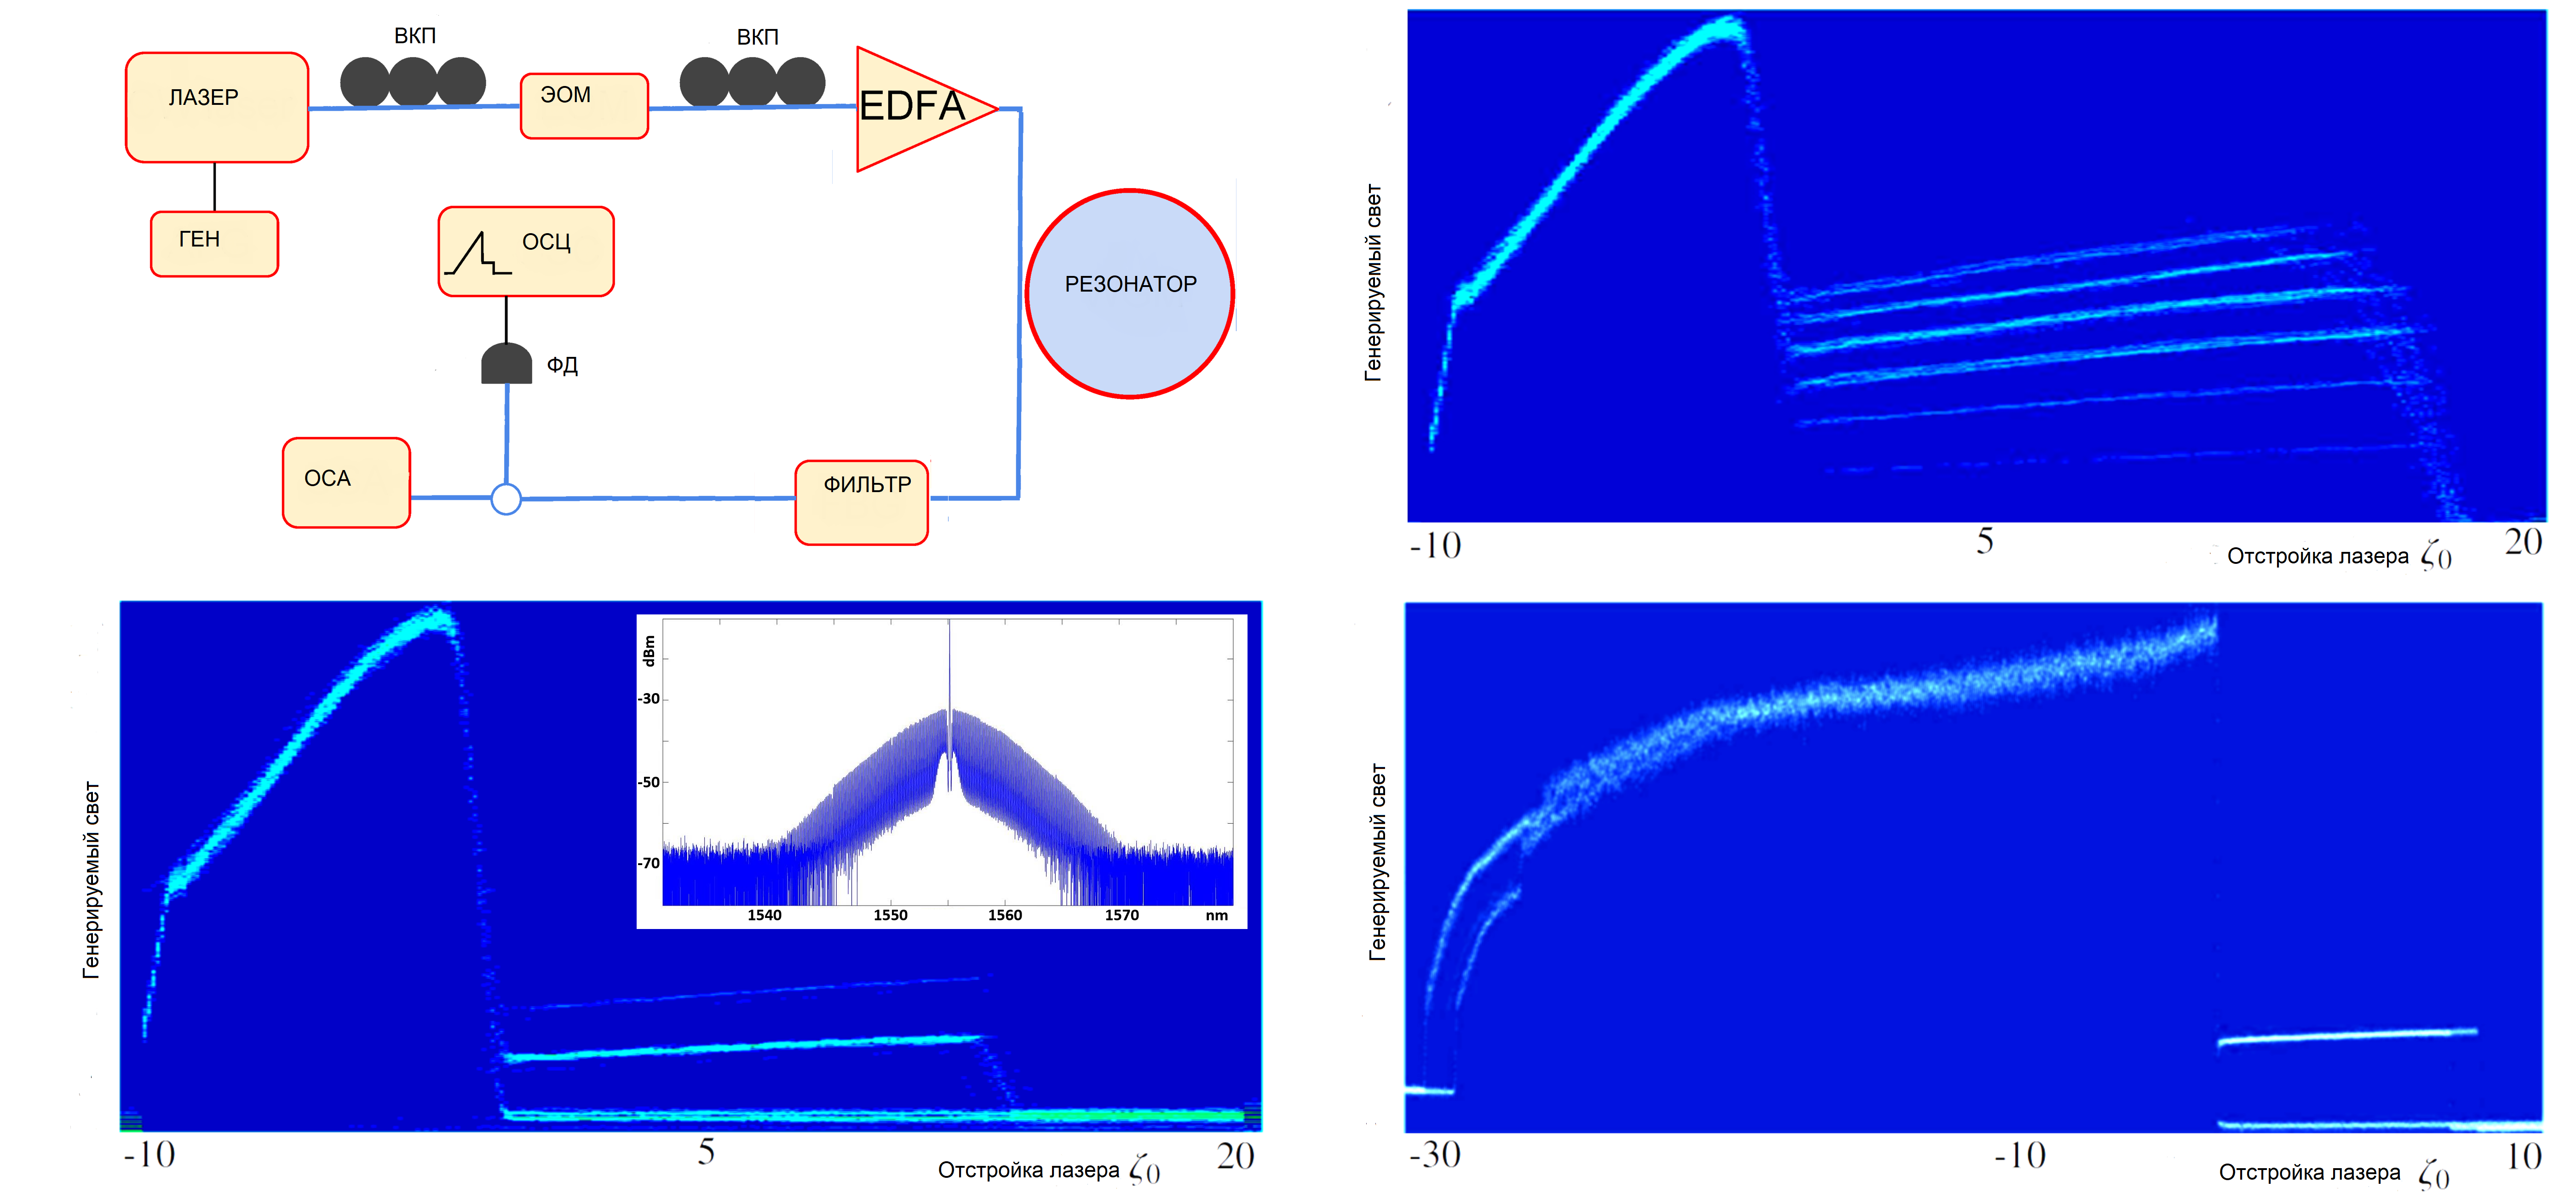
\includegraphics[width=1\linewidth]{Experiment_s}
  \caption{Экспериментальное измерение формирования солитонов при фазовой модуляции накачки и сканировании лазера. (a) экспериментальная установка (AFG, генератор сигналов произвольной формы; CW laser, узкополосный перестраиваемый лазер непрерывной мощности; FPC, волоконный контроллер поляризации, EDFA, эрбиевый волоконный усилитель; WGM,  микрорезонатор из MgF$_2$; FBG, волоконный Брэгговский фильтр; PD, фотодиод; OSA, оптический спектроанализатор; OSC, осциллограф); (b) статистика 100 измерений по осциллографу сканирования лазера нелинейной моды резонатора на частоте 100 Гц, показана зависимость генерируемого света от отстройки частоты лазера без внешней модуляции, (c) статистика при включенной фазовой модуляции, частота сканирования лазера 100 Гц, вероятность отсутствия солитонов - 0.5, генерации 1 солитона - 0.4, двух солитонов - 0.1, вставка показывает оптический спектр односолитонного режима с $\text{sech}^2(x)$ огибающей, ширина спектра 35 нм, расстояние между линиями соответствует 1 ОСД резонатора в 12.1 ГГц; (d) статистика 100 измерений при включенной амплитудной модуляции, частота сканирования лазера 5 Гц, вероятность отсутствия солитонов - 0.4, генерации 1 солитона - 0.6.}
  \label{chaos_order_experiment}
\end{figure}

Накачивая резонатор лазером мощностью 100 мВт после усилителя на длине волны 1554 нм наблюдаются характерные ступеньки в сигнале генерируемого света, соответствующие формированию солитонов. Оптический спектр односолитонного режима приведен на вставке рис. \ref{chaos_order_experiment}(c).

Экспериментально были проверены разные разные скорости сканирования частоты лазера от 0.25 ГГц/с до 25 ГГц/с ($\alpha \approx 0.0006...0.06$). Одновременно была приложена либо фазовая либо амплитудная модуляция накачки с помощью волоконного электрооптического модулятора. Глубина амплитудной и фазовой модуляции была около -26 дБн ($\varepsilon \approx 0.1$). Для анализа были записаны по 100 сигналов с фотодектора для каждого набора параметров.

Рис. \ref{chaos_order_experiment}(b)-\ref{chaos_order_experiment}(d) показывает наложенные друг на друга данные от 100 измерений, демонстрируя статистику генерации солитонов, т.ч. более яркие кривые означают более высокую вероятность такого сценария. Было обнаружено, что оптимальная частота модуляции, при которой наблюдался наиболее вероятный односолитонный режим была близка, но не совпадала точно с частотой $12.1025$ ГГц - ОСД "горячего" резонатора, который был измерен по сигналу биений в солитонном режиме. Оптимальное отличие частоты модуляции от этого значения ФСР составило около 1 МГц. При этом отклонение частоты от оптимальной более, чем на 100 кГц приводило к исчезновению эффекта более вероятной односолитонной генерации. Такое отклонение оптимально частоты от ОСД может быть объяснено тем, что ОСД холодного резонатора из численной модели отличается от измеренного ОСД нагретого резонатора в эксперименте. Из экспериментальных данных видно, как фазовая так и амплитудная модуляция накачки радикально меняется распределение вероятностей для числа генерируемых солитонов, т.ч. односолитонный режим становится достижимым и наиболее вероятным. Хотя эксперимент хорошо качественно согласуется с численным моделированием, видны отличия из-за неучтенных эффектов, вызванных дисперсией более высокого порядка и тепловыми эффектами.

\subsection{Исследование зависимости свойств свойств солитонов от отстройки лазера накачки}


\section{Исследование метода стабилизации частоты повторения солитона} 

Пример нестабильности частоты повторения солитона без стабилизации отстройки дан на рис. \ref{beatnote_drift_2min} и составляет порядка 5 кГц за 2 мин.

\begin{figure}[ht]
\centering
  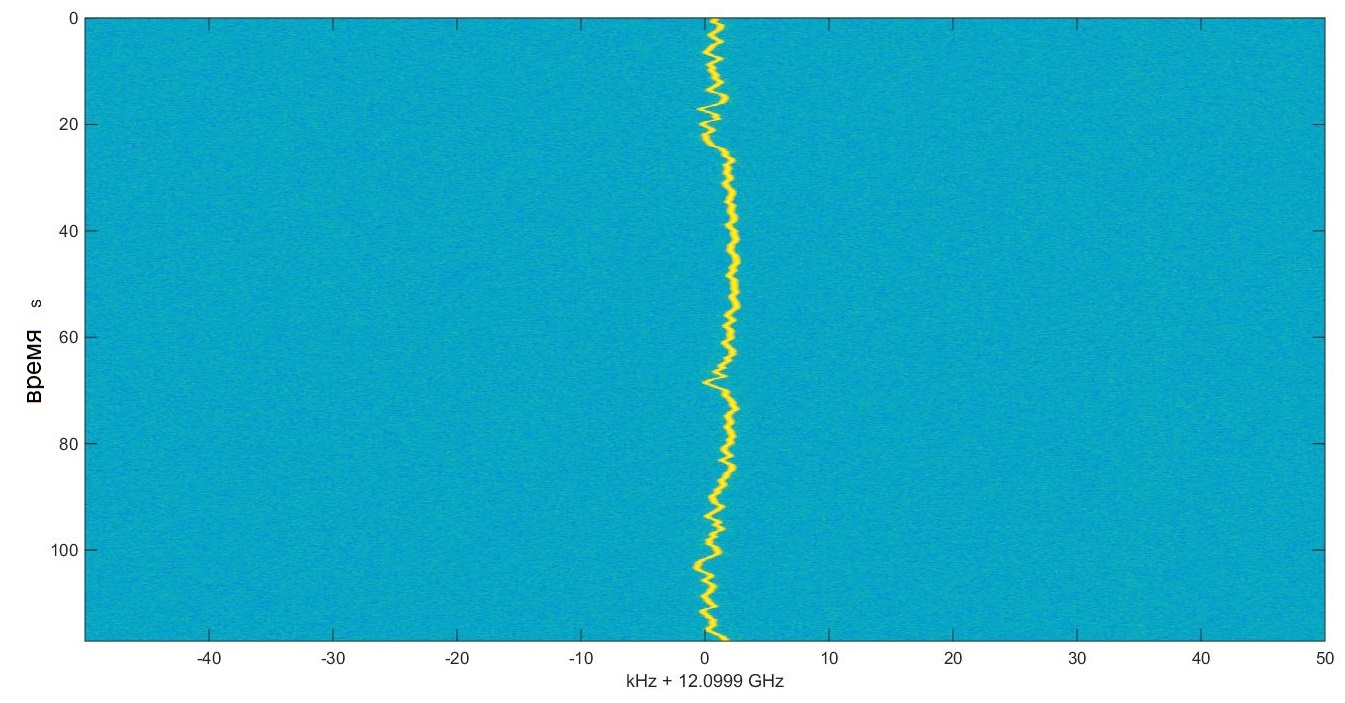
\includegraphics[width=0.5\linewidth]{beatnote_drift_2min}
  \caption{Нестабильности частоты повторения солитона без стабилизации отстройки за 2 мин порядка 5 кГц}
  \label{beatnote_drift_2min}
\end{figure}



\section{Экспериментальное наблюдение вынужденного рассеяния Рамана и Бриллюэна в кристаллических микрорезонаторах}

Суммарная (материальная + геометрическая) ДГС резонатора из $BaF_2$ является нормальной на 1550 нм \cite{}, поэтому генерация светлых солитонов невозможна. При исследовании резонаторов из $BaF_2$ при накачке на длине волны 1550 нм наблюдались эффекты вынужденного рассеяния Рамана и Бриллюэна.

Фторид бария имеет отрицательный терморефрактивный ($-19\times10^{-6}/C^{o}$) и положительный термоэластичный коэффициенты ($18.1\times10^{-6}/C^{o}$). При накачке большой оптической мощностью наблюдались периодические термооптические осцилляции, которые не позволяют настроить частоту лазера на моду (Рис. \ref{baf_thermoptic}). При настройке лазера на моду резонатора объем моды нагревается быстро, потом диффузией тепло распространяется в объеме всего кристаллического диска. Сдвиг частоты моды происходит из-за зависимости показателя преломления от температуры (терморефрация), а также из-за теплового расширения материала. Пусть сначала лазер строго в резонансе с модой резонатора. Объем моды быстро нагревается, температура увеличивается и резонанс сдвигается в синюю сторону (в область более высоких частот) из-за терморефракции. Лазер перестает накачивать моду, объем моды остывает, тепло распространяется по объему всего диска, он расширяется, сдвигая собственную частоту мод в красную сторону, лазер медленно начинает разогревать моду. Мода при этом выглядит как стандартная нелинейная мода с тепловой нелинейностью при сканировании частоты, далее на определенной отстройке лазер срывается с нелинейной моды. Далее объем всего резонатора начинает остывать, моды сдвигаются и через определенное время лазер заново начинает заходить в моду но со стороны красной отстройки. Процесс периодически повторяется. Важно отметить, что при использовании электрической схемы привязки частоты лазера PDH, и плавном увеличении мощностью лазер можно привязать к нелинейной моде $BaF_2$ на длительное время.

Отметим, что для связи с резонатором из $BaF_2$ при накачке на длине волны 1550 нм с показателем преломления $n=1.4661$ использовалось растянутое волокно SMF28 из плавленого кварца с $n=1.452$ для ядра волокна. В теории элемент связи должен иметь больший показатель преломления, чем материал для эффективной связи. Однако экспериментально изготовить растянутое волокно для связи с резонатором из фторидом бария оказалось даже легче, чем для связи с резонатором из фторида магния, т.к. даже при толщине волокна порядка 7-8 мкм уже наблюдалась связь. Также была достигнута критическая связь с растянутым волокном.

\begin{figure}[ht]
\begin{minipage}[ht]{0.49\linewidth}\centering
    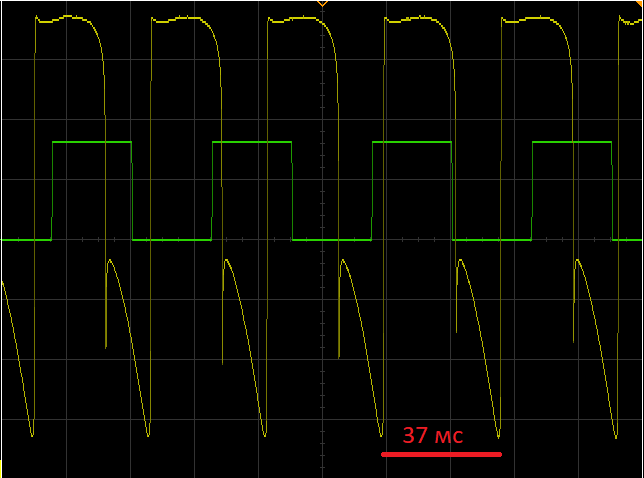
\includegraphics[width=1\linewidth]{baf_thermoptic}
  \end{minipage}
  \hfill
  \begin{minipage}[ht]{0.49\linewidth}\centering
    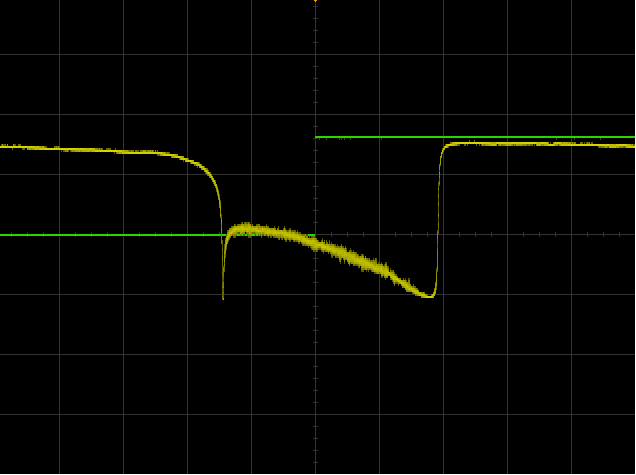
\includegraphics[width=1\linewidth]{baf_themoopticsingle}
  \end{minipage}
    \caption{Термооптические осцилляции в резонаторе $BaF_2$ диаметром 1 мм при накачке мощностью 25 мВт.}
  \label{baf_thermoptic}
\end{figure}

При диаметре резонатора из $BaF_2$ 400 мкм, и радиусе кривизны 100 мкм (ОСД 162.7 GHz и расстояние между линиями гребенки 1.3 нм) геометрическая дисперсия уже компенсирует нормальную материальную дисперсию и суммарная дисперсия нормальная. Поэтому удалось наблюдать каскадную генерацию нескольких линий гребенки на значительном удалении от моды накачки и одновременно генерацию вынужденного рамановского излучения на длине волны 1615 нм, что соответствует табличному значению для рамановского сдвига в материале \ref{baf_comb_anomal}.
 
\begin{figure}[ht]
\begin{minipage}[ht]{0.49\linewidth}\centering
    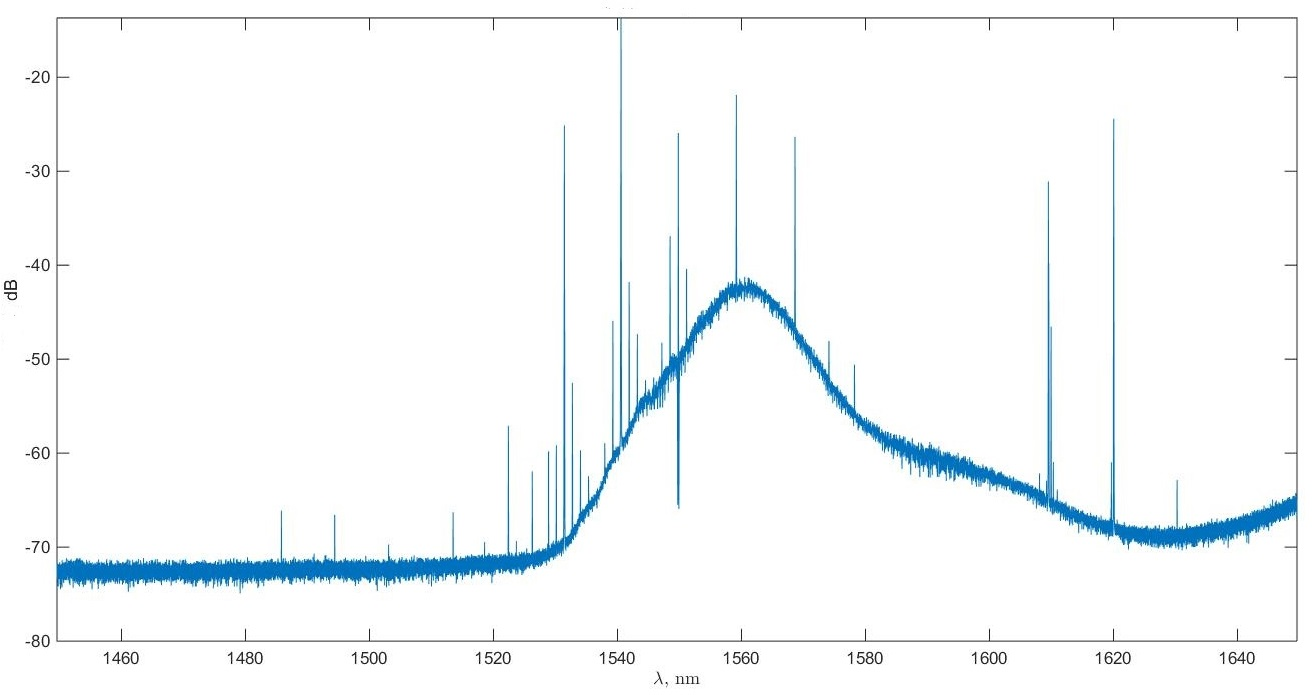
\includegraphics[width=1\linewidth]{b44_3}
  \end{minipage}
  \hfill
  \begin{minipage}[ht]{0.49\linewidth}\centering
    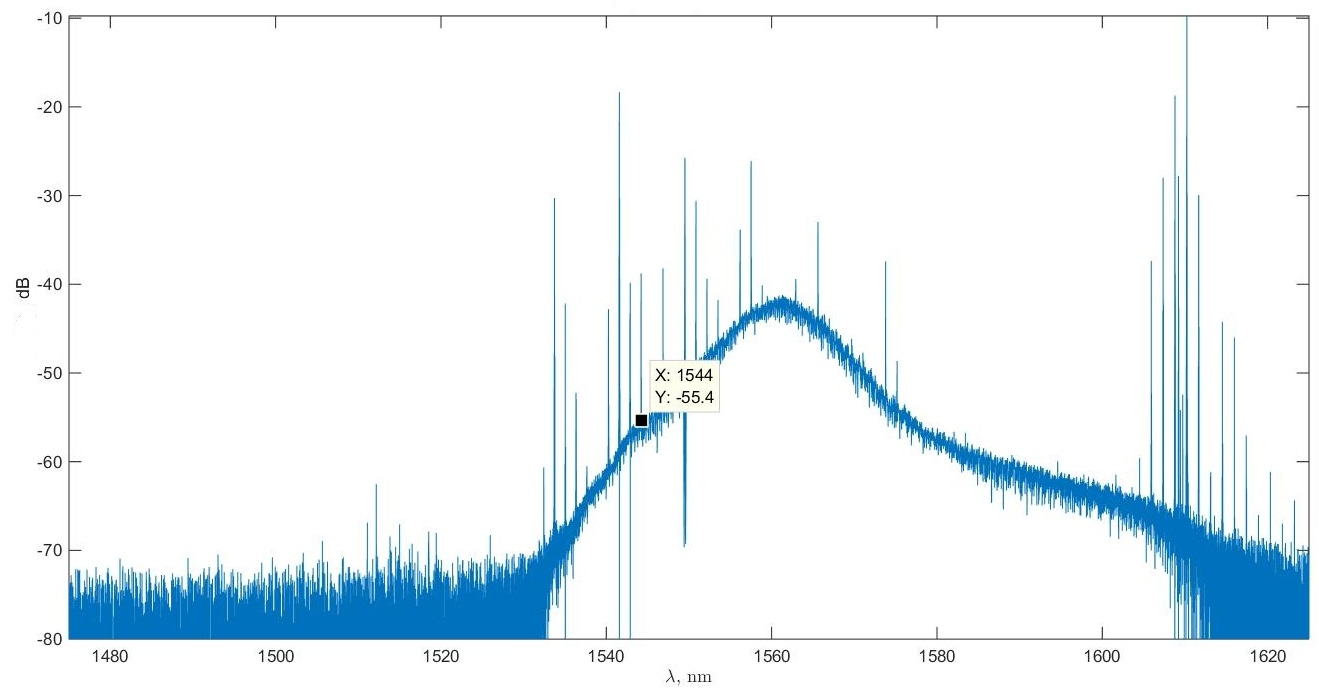
\includegraphics[width=1\linewidth]{b44_4}
  \end{minipage}
    \caption{Оптический спектр вынужденного Рамановского рассеяния и генерации оптической гребенки в резонаторе $BaF_2$ диаметром 400 мкм при аномальной дисперсии групповой скорости.}
  \label{baf_comb_anomal}
\end{figure}

В другом резонаторе из $BaF_2$ с диаметром 3.9 мм, ОСД 16.689 ГГц, с радиусом кривизны 500 мкм существенно больше мод, они расположены близко друг к другу и при большой мощности в нелинейном режиме перекрываются. Бриллюэновская частота не совпадает с ОСД фундаметального семейства мод (16.689 ГГц). Резонансное рассеяние света на акустических колебаниях кристаллической решетки происходит в ширине полосы Бриллюэна и усиление просходит на модах из другого семейства. Бриллюэновский сдвиг вычисляется как $\nu_b=2*n_{eff}*V_a/\lambda$, где $V_a$ вычисляется через эластичные константы и плотность материала. Для накачке на длине волны 1550 нм расчетное значение $\nu_b=8.27$ ГГц. Ширина полосы усиления достаточна мала и составляет порядка 10 МГц, поэтому необходимо иметь высокодобротную моду резонатора в этом диапазоне для усиления. В исследуемом резонаторе соответственно больше мод, чем в резонаторе меньшего в 10 раз диаметра, на которых наблюдается вынужденной рассеяние Бриллюэна (ВРБ), каскадно при мощности накачки в эксперименте в 25 мВт. Порог по мощности для наблюдения первого пика ВРБ был около 8 мВт, что существенно выше, чем в работах с Бриллюэновским лазером. Это связано с сравнительно невосокой добротностью мод резонатора $1*10^8$. В эксперименте наблюдались пики каскадного ВРБ на 8.2, 16.4, 24.6 ГГц нечетные пики в отраженной волне, четные в проходящей \ref{baf_sbs}. Нечетные пики измерялись в отраженной волне на выходе оптического циркулятора, поставленного до элемента связи с резонатором. Усредненная ширина биений на частоте Бриллюэновского рассеяния составила около 2 МГц, такая большая ширина объясняется тем, что лазер накачки не был привязан по частоте к моде резонатора, и фактически сбор данных происходил при усреднении за большое время, по периодическим термоосцилляциям моды резонатора.

Отдельно была предпринята попытка изготовить резонатор такого диаметра, что удвоенная частота ВРБ (16.39-16.43 ГГц измеренная в предыдущем эксперименте) совпадала с ОСД резонтора. Такой резонатор был изготовлен, однако в экспериментах с ним никакой новой динамики наблюдать не удалось.

\begin{figure}[ht]
\begin{minipage}[ht]{0.49\linewidth}\centering
    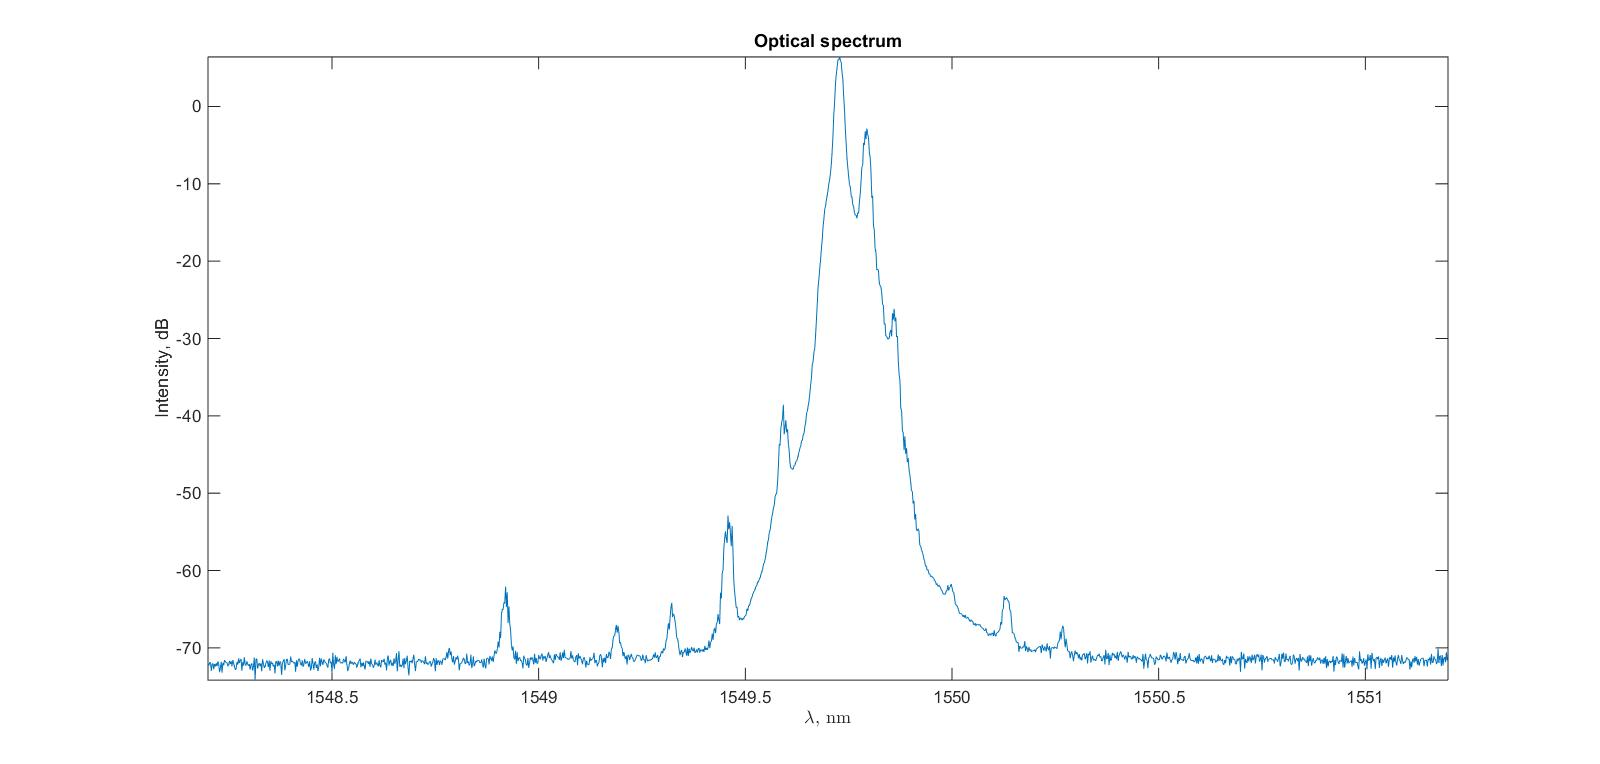
\includegraphics[width=1\linewidth]{baf_sbs_cascaded_osa}
  \end{minipage}
  \hfill
  \begin{minipage}[ht]{0.49\linewidth}\centering
    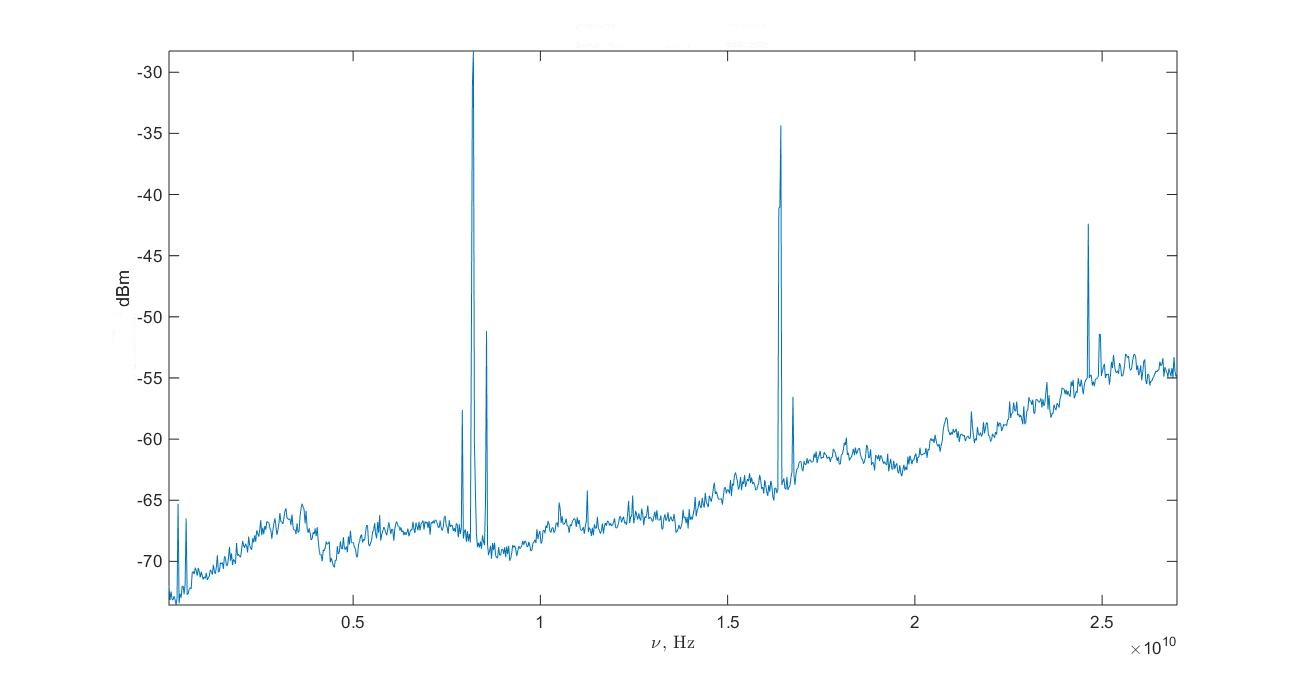
\includegraphics[width=1\linewidth]{baf_sbs_cascaded_esa}
  \end{minipage}
    \caption{Слева: оптический спектр каскадного вынужденного Бриллюэновского рассеяния в резонаторе $BaF_2$ диаметром 3.9 мкм. Дисперсия резонатора нормальна, широкой керровской гребенки не наблюдалось. Справа: сигнал биений на частоте ВРБ и гармониках 8.2, 16.4, 24.6 ГГц, шириной около 2 МГц.}
  \label{baf_sbs}
\end{figure}

При исследовании резонаторов из $MgF_2$ при накачке на длине волны 1300 нм, где суммарная ДГС резонатора была нормальной, была произведена попытка наблюдать генерацию оптических частотных гребенок при нормальной дисперсии с помощью двухчастотной накачки с разницей частот строго совпадающей с ОСД резонатора. Однако выходная мощность в схеме с имеющимся лазером и амплитудным электрооптическом модулятором (не волоконного, а на свободных пучках в пространстве) была недостаточна для преодоления порога по мощности. Однако впервые было наблюдено вынужденное Рамановское рассеяние в резонаторе из $MgF_2$ \ref{mgf_srs}, что никогда не удавалось сделать при накачке на 1550 нм при различных поляризациях. Рамановский сдвиг хорошо совпадает по частоте с табличным значением. На фотодетекторе с полосой 25 ГГц наблюдался только сигнал на частоте межмодового расстояния резонатора. Два близких пика имели ширину около 200 кГц при усреднении. \ref{mgf_srs_beatnote}. Можно предположить на основе огибающей линий в оптическом диапазоне рамановсого усиления, что возбуждались линии другого семейства, но с близкими собственными частотами. Отметим, что используемый лазер накачки имел собственную ширину линии много больше, чем ширина линии микрорезонатора, поэтому невозможно было эффективно накачать моду резонатора и стационарная картина генерации гребенки не наблюдалась, дополнительных схем стабилизации частоты не применялось.

Отдельно стоит отметить, что в многочисленных экспериментах с резонаторами из $MgF_2$ разного размера и формы, при накачке на длинах волнах 1.5, 1.65 мкм никогда не наблюдалось вынужденное рассеяние Бриллюэна ни при какой поляризации лазера накачки.

\begin{figure}[ht]
\begin{minipage}[ht]{0.49\linewidth}\centering
    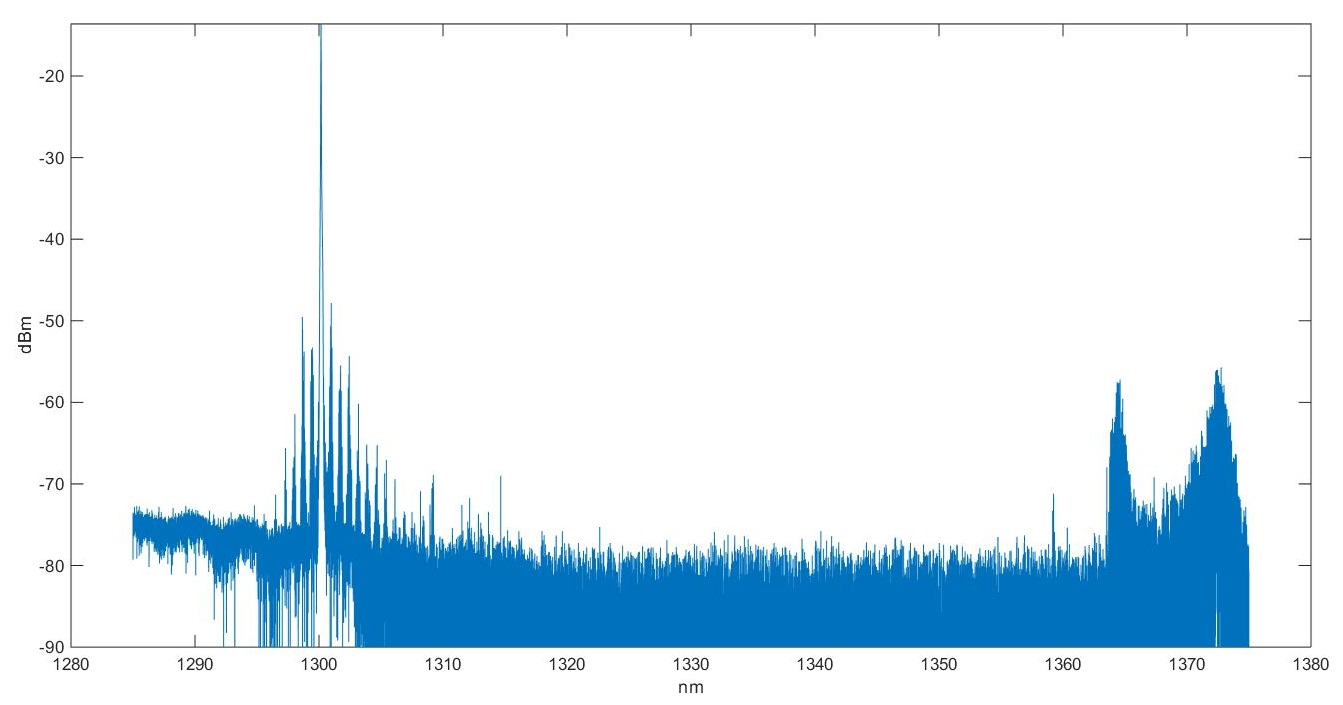
\includegraphics[width=1\linewidth]{comb1330nm_raman}
  \end{minipage}
  \hfill
  \begin{minipage}[ht]{0.49\linewidth}\centering
    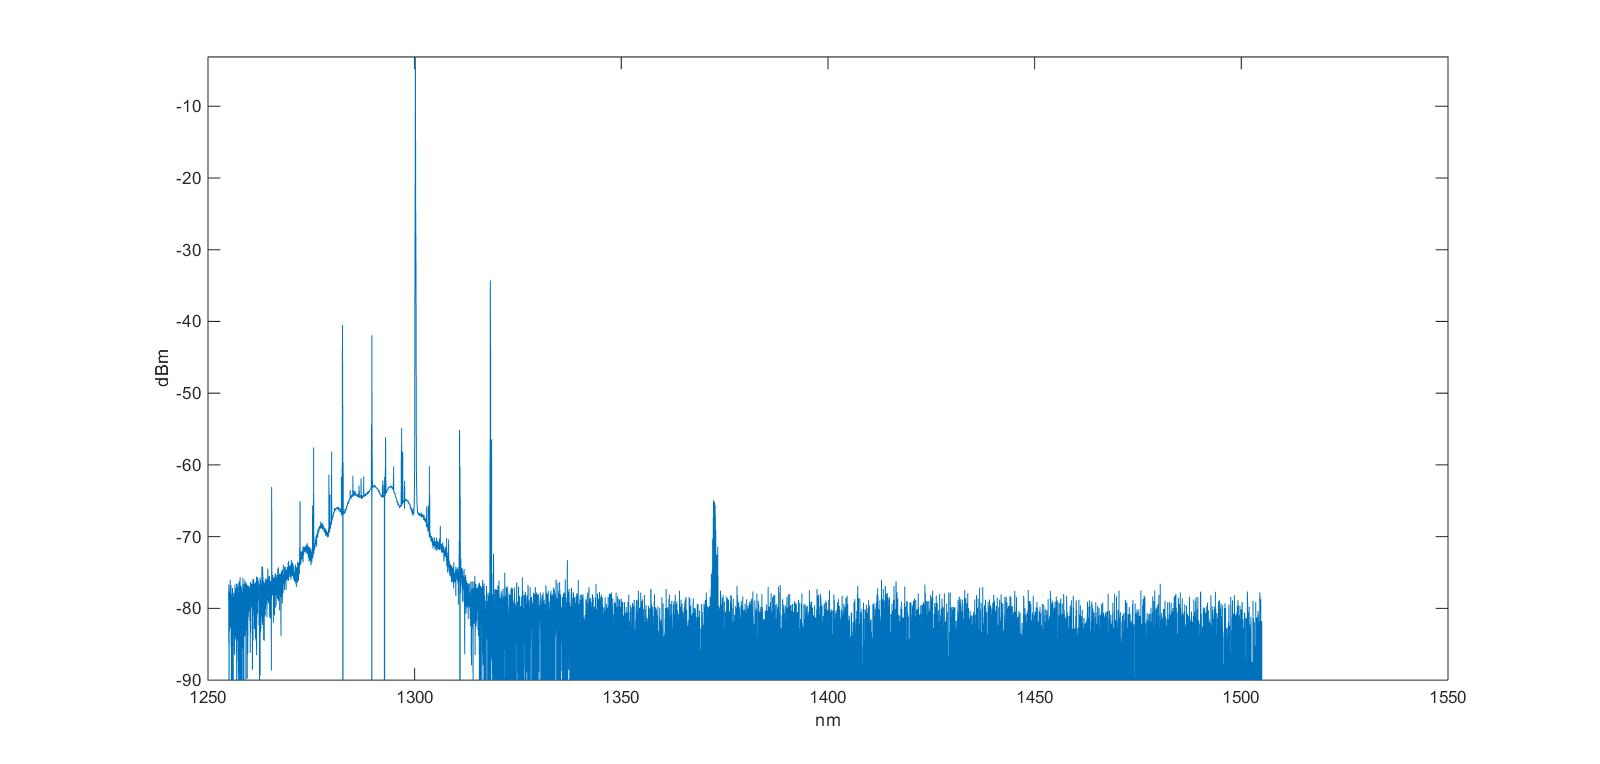
\includegraphics[width=1\linewidth]{comb1330nm_raman2}
  \end{minipage}
    \caption{Оптические спектры вынужденного Рамановского рассеяния в резонаторе $MgF_2$ диаметром 5 мм, ОСД 12.1 ГГц, приводящие к генерации некогерентной оптической гребенки около накачки на 1300 нм, в области нормальной дисперсии резонатора. Мощность накачки 30 мВт. Слева и справа - разные накачиваемые моды.}
  \label{mgf_srs}
\end{figure}

\begin{figure}[ht]
\begin{minipage}[ht]{0.49\linewidth}\centering
    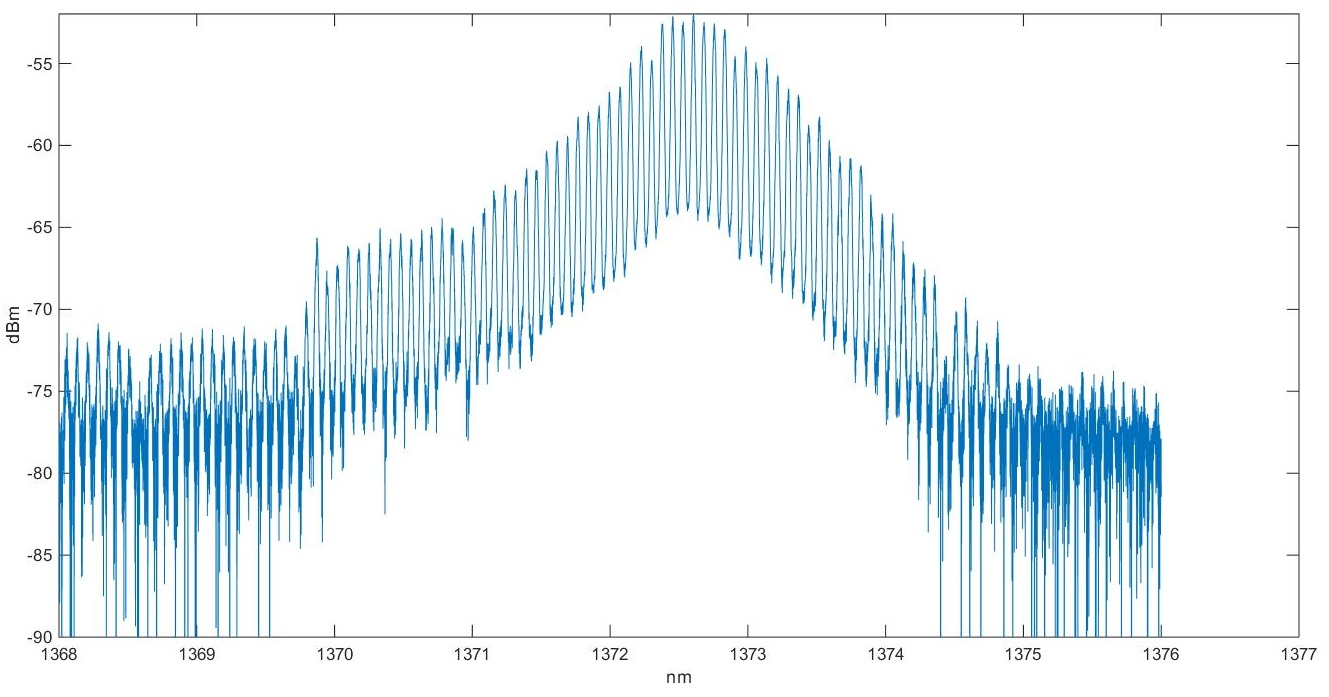
\includegraphics[width=1\linewidth]{raman_srs_zoomed}
  \end{minipage}
  \hfill
  \begin{minipage}[ht]{0.49\linewidth}\centering
    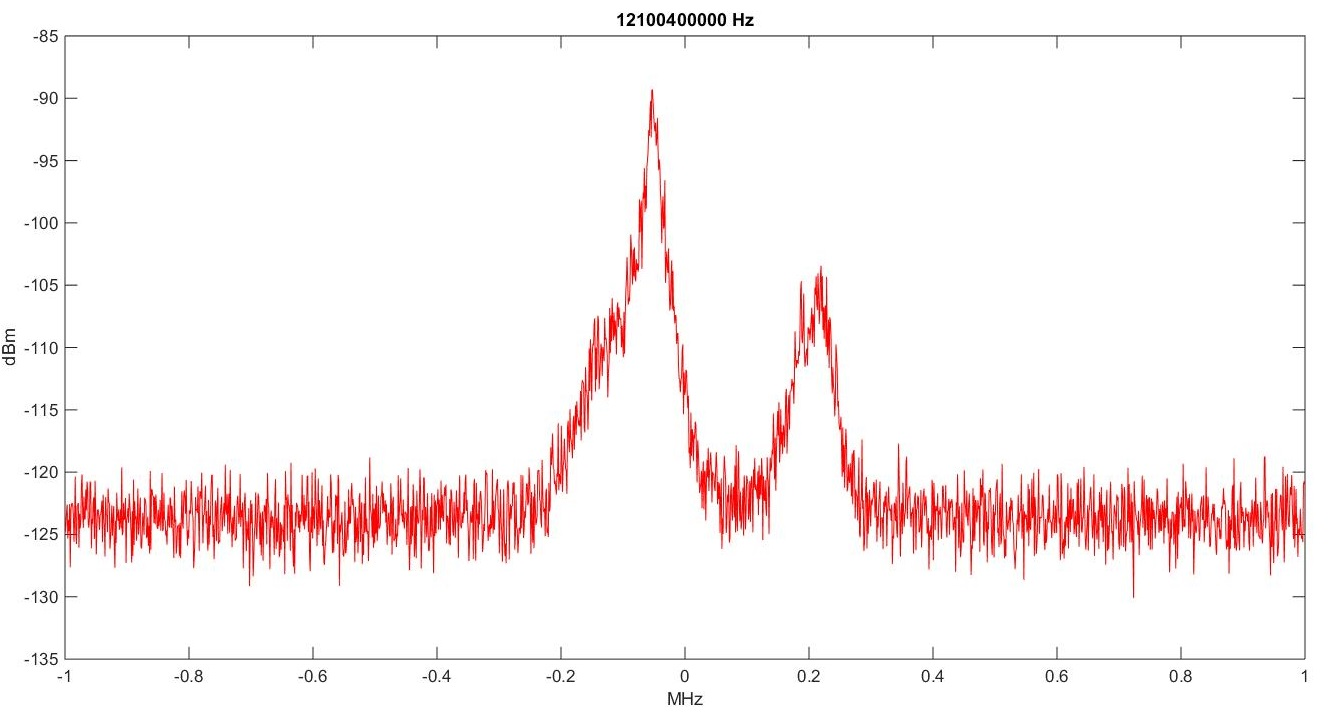
\includegraphics[width=1\linewidth]{raman_mgf_esa_beatnote}
  \end{minipage}
    \caption{Слева: Оптический спектр полосы рамановского усиления в резонаторе $MgF_2$ при накачке на 1300 нм. Справа: спектр биений на частоте межмодового расстояния резонатора 12.1 ГГц, ширина линий около 200 кГц}
  \label{mgf_srs_beatnote}
\end{figure}


%Сошлемся на все конференции \cite{confbib1,confbib2,confbib3,confbib4,confbib5,confbib6,confbib7,confbib8,confbib9,confbib10,confbib11,confbib12,confbib13,confbib14}
